This section presents verification and performance results of the standard and hybrid FEM-BEM coupling schemes, for molecules modeled as cavities with constant and varying permittivity.
When the permittivity inside the molecule was constant, we tested convergence against the available analytical expression of the solvation energy of a sphere [Kirkwood1934], and then compared a more realistic geometry (arginine) with a purely BEM implementation.
On the other hand, we considered a Gaussian-varying permittivity [Alexov and earlier] inside arginine, and used APBS [Baker2001] to verify.
The final result of this section shows the scaling of the standard and hybrid FEM-BEM coupling, as the molecule size grows. 

All runs were done on XX computer with YY specifications. 

\section*{\sffamily \Large Results with constant permitivitty}

In implicit-solvent models, the molecule is usually considered as a region with constant permittivity, in this case, with $\epsilon_1=4$.
In the solvent region, we used the permittivity of water ($\epsilon_2$=80) and an inverse of the Debye length of $\kappa=0.125$ \AA$^{-1}$.

\subsection*{\sffamily \large Convergence of a spherical cavity}

The Kirkwood sphere [Kirkwood1934] is a standard benchmarck for the Poisson-Boltzmann equation in molecular electrostatics. 
Here, we considered a spherical cavity with radius $R=X$ \AA, with three charges ($q_1$=a, $q_2$=b, and $q_3$=c) placed at $\mathbf{x}_1=(x_1,y_1,z_1)$, $\mathbf{x}_2=(x_2,y_2,z_2)$, and $\mathbf{x}_3=(x_3,y_3,z_3)$, which has an exact $\Delta G_{solv}=XX$ kcal/mol.
Figure \ref{fig:error_sphere} shows the error convergence of the standard and hybrid FEM-BEM approaches, and a reference BEM implementation, to the analytical solution. 
In these runs, the FEM mesh was generated from a surface mesh with W, X, Y, and Z vertices per \AA$^2$ on the SES, which was also used for the BEM runs. 
The error in Figure \ref{fig:error_sphere} decays linearly with the surface area, which agrees with the expected convergence for P1 elements, indicating a correct implementation of the numerical scheme. 

\begin{figure}
  \centering
  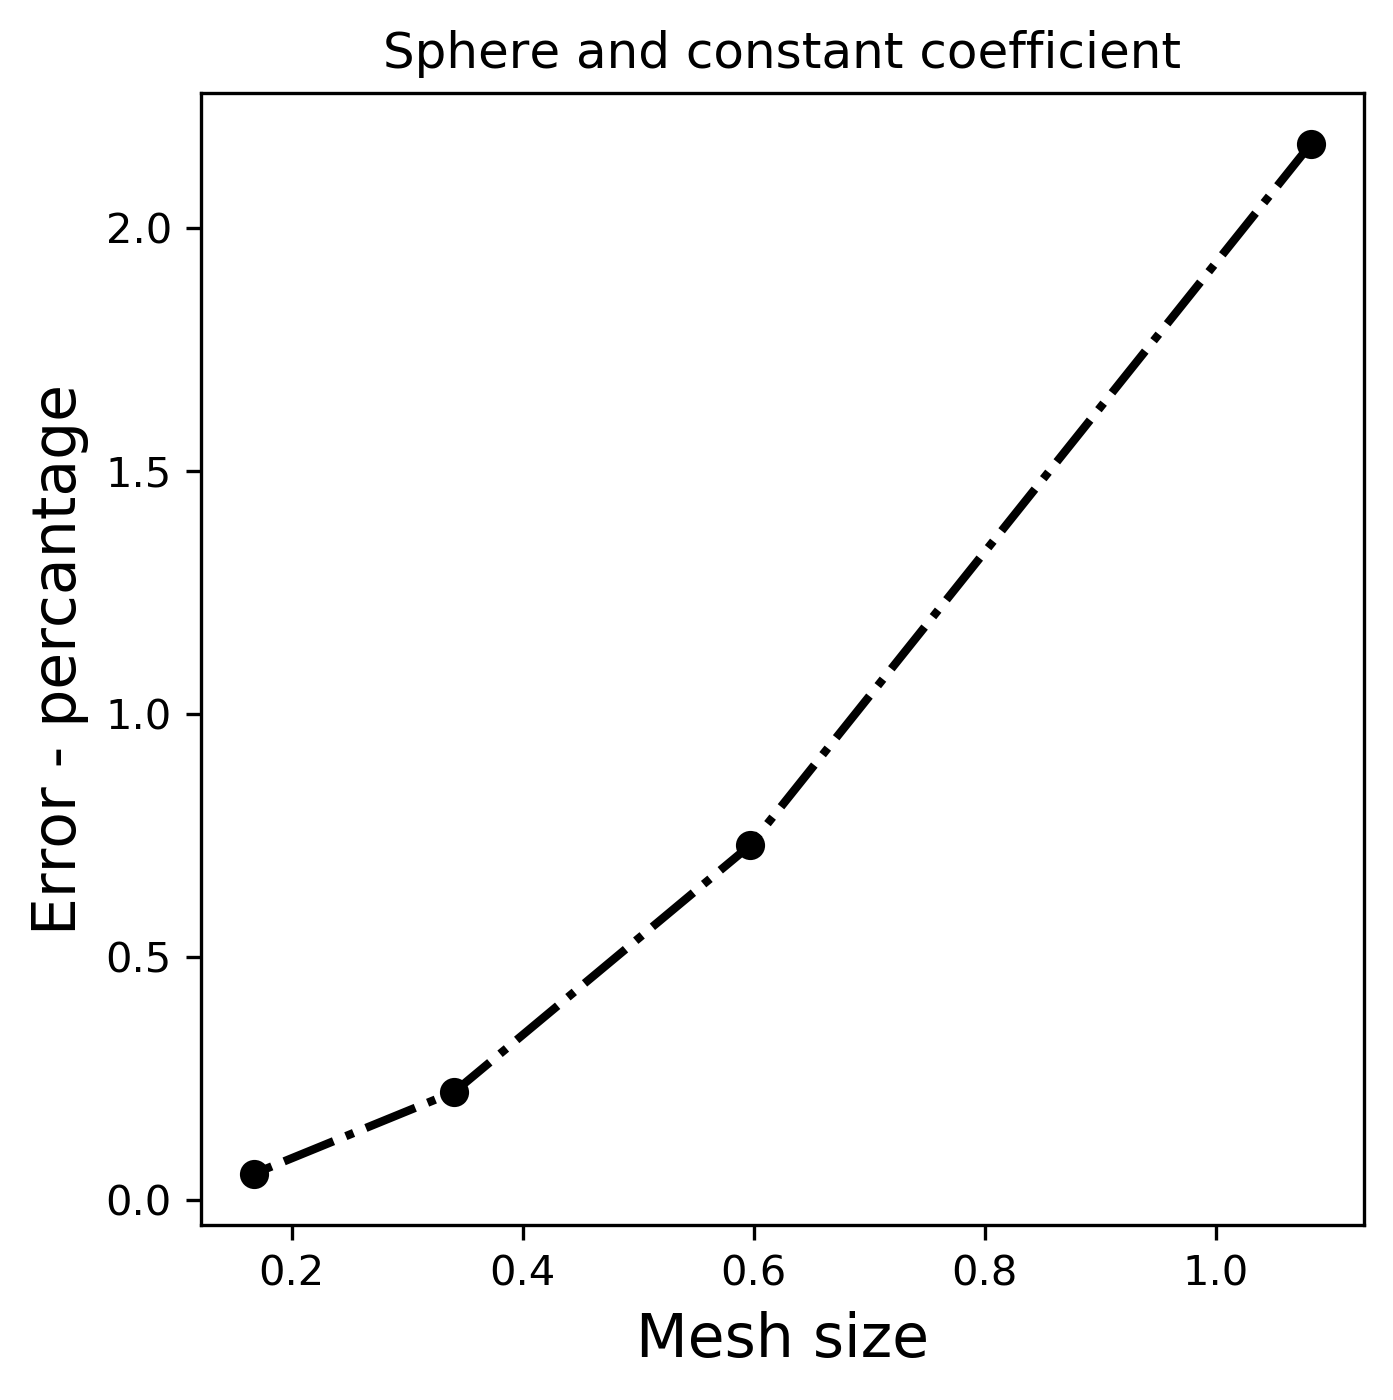
\includegraphics[width=0.45\linewidth]{BEM_BEM_Sphere_const_coeff_error.png}
  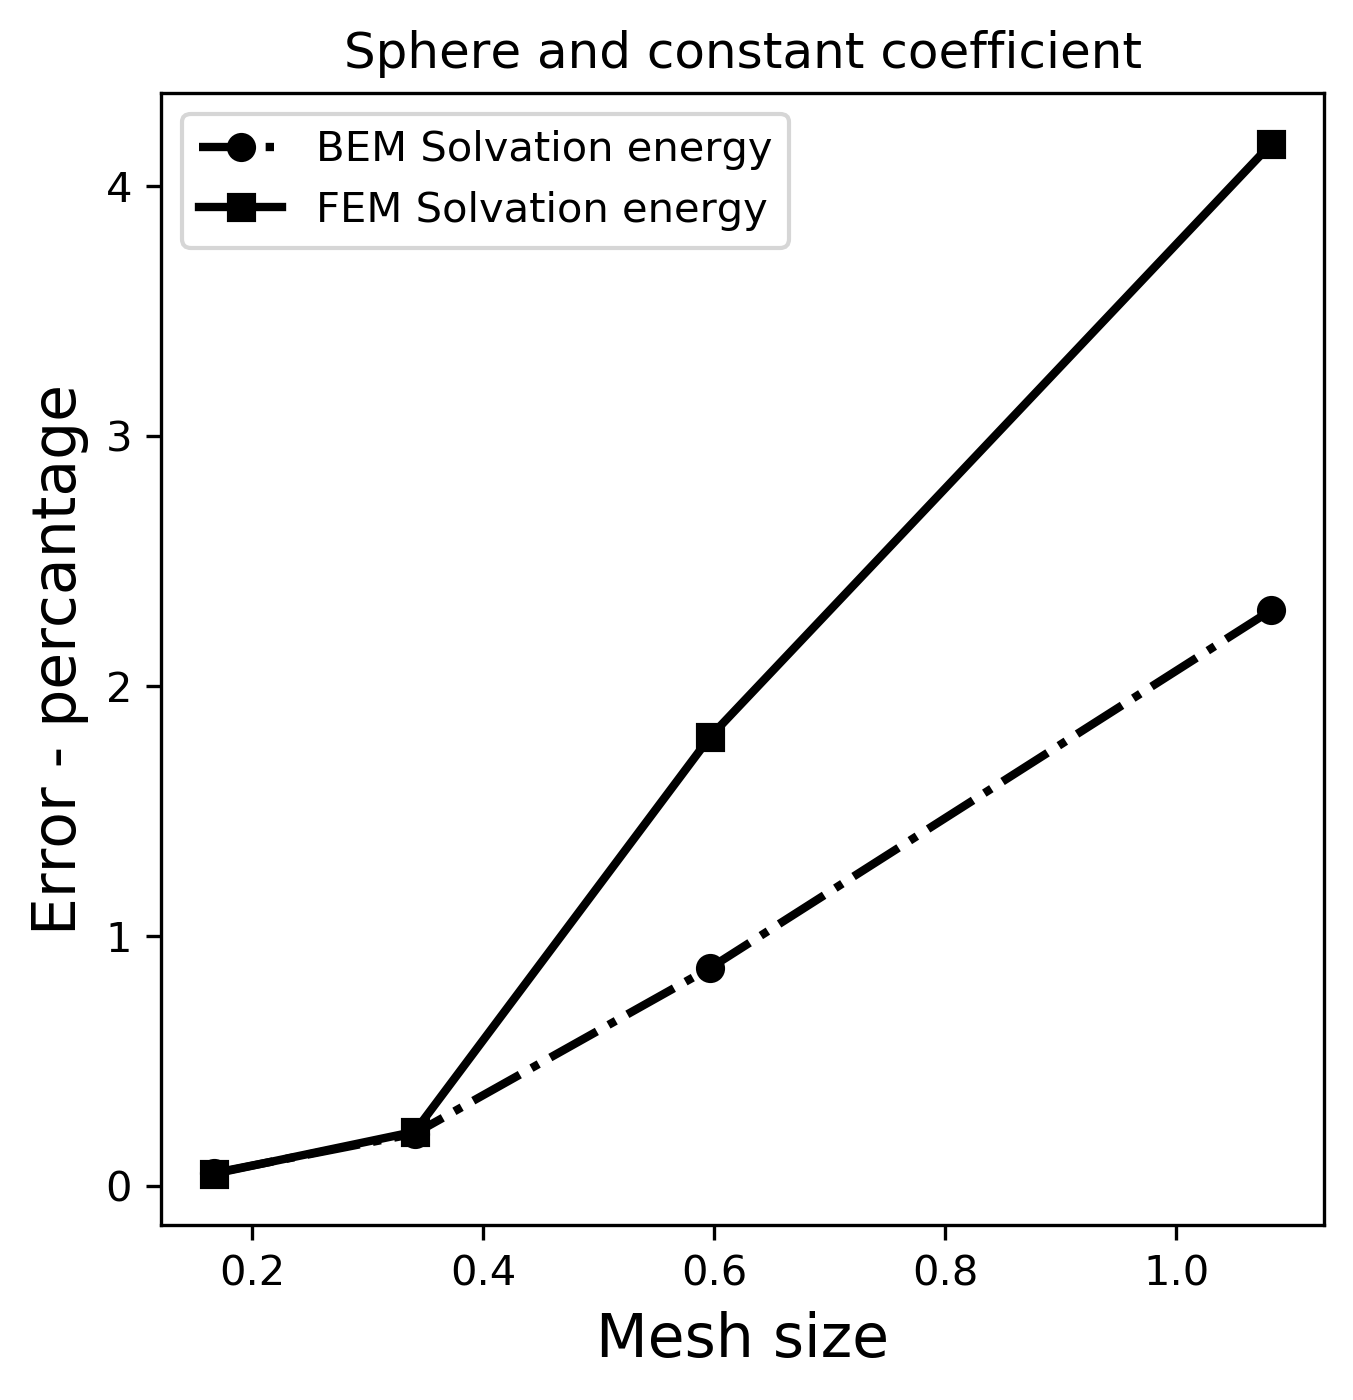
\includegraphics[width=0.45\linewidth]{FEM_BEM_Sphere_const_coeff_error.png}
  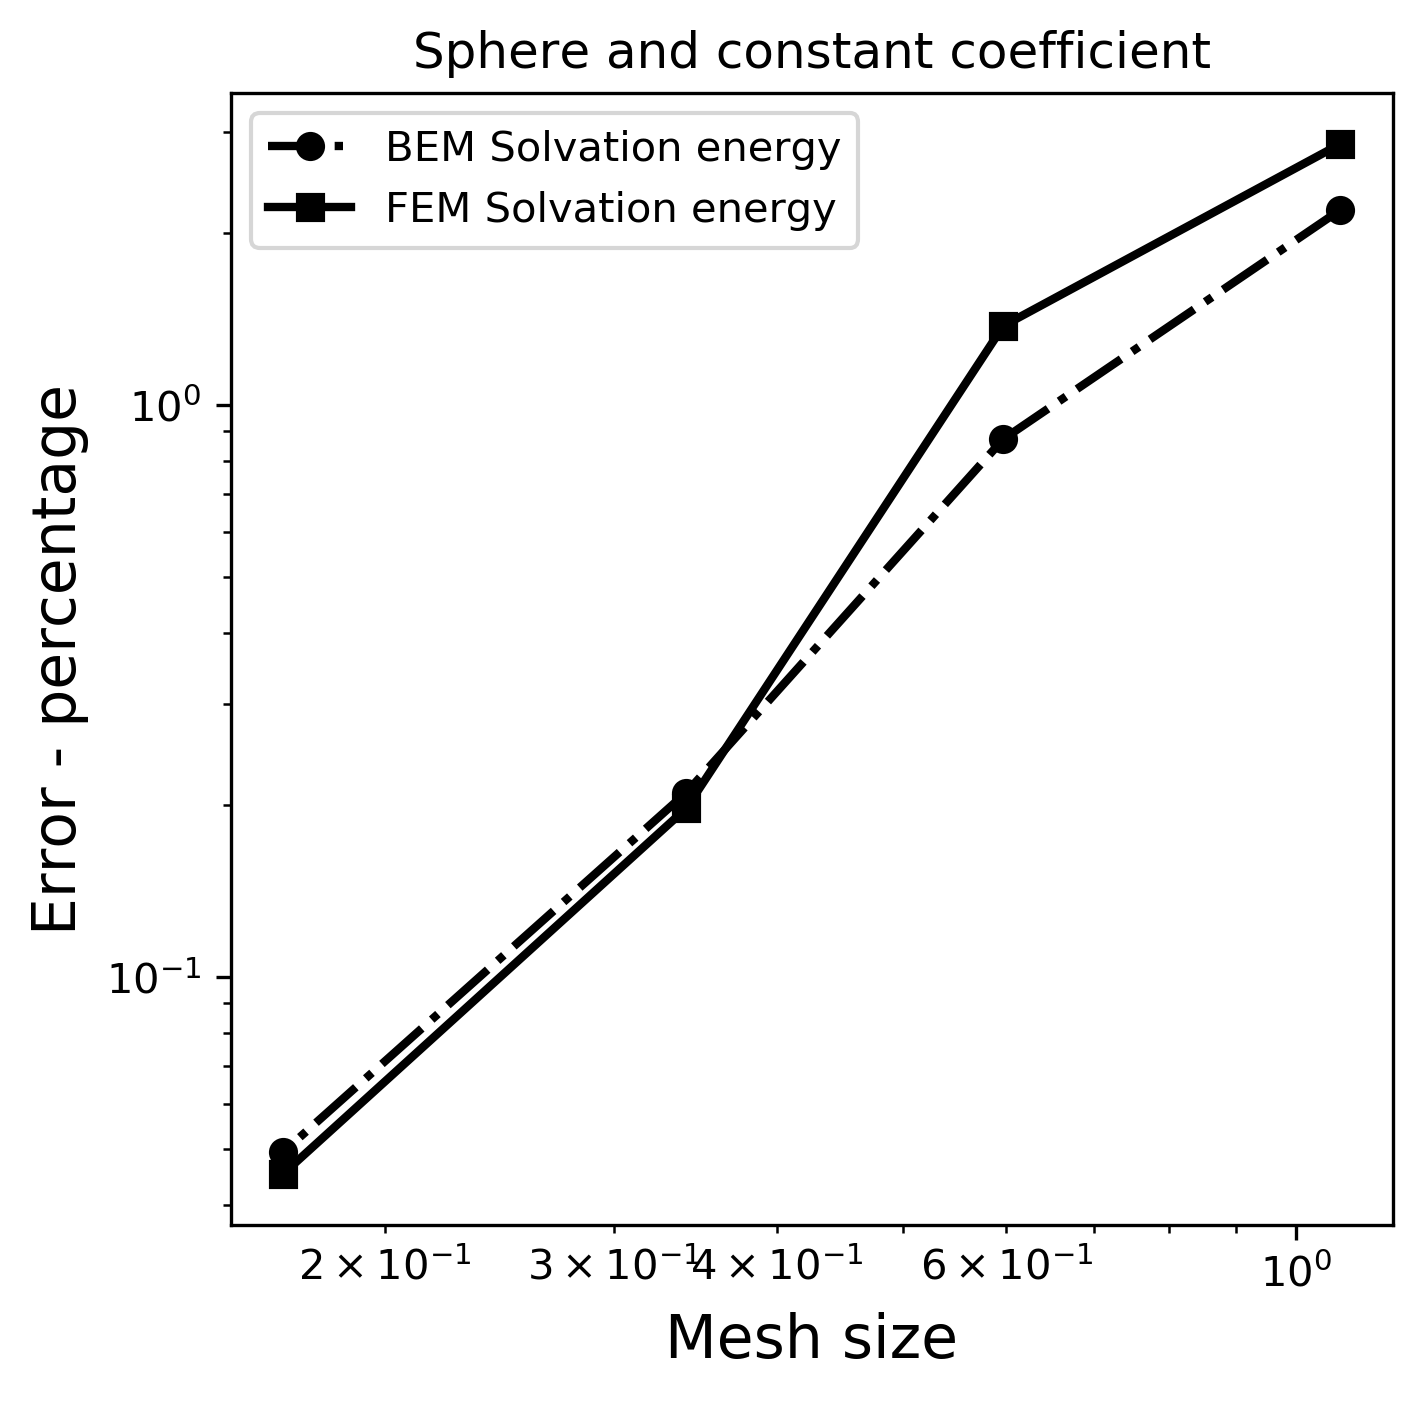
\includegraphics[width=0.45\linewidth]{Hybrid_FEM_BEM_Sphere_const_coeff_error.png}
  \caption{Error for the Kirkwood sphere. Can we put all these in a single plot and in log-log?}
  \label{fig:error_sphere}
\end{figure}

%\begin{itemize}
%    \item Show convergence to analytical solution for
%    \begin{itemize}
%        \item BEM-BEM
%\begin{figure}[!htb]
%\minipage{0.32\textwidth}
%  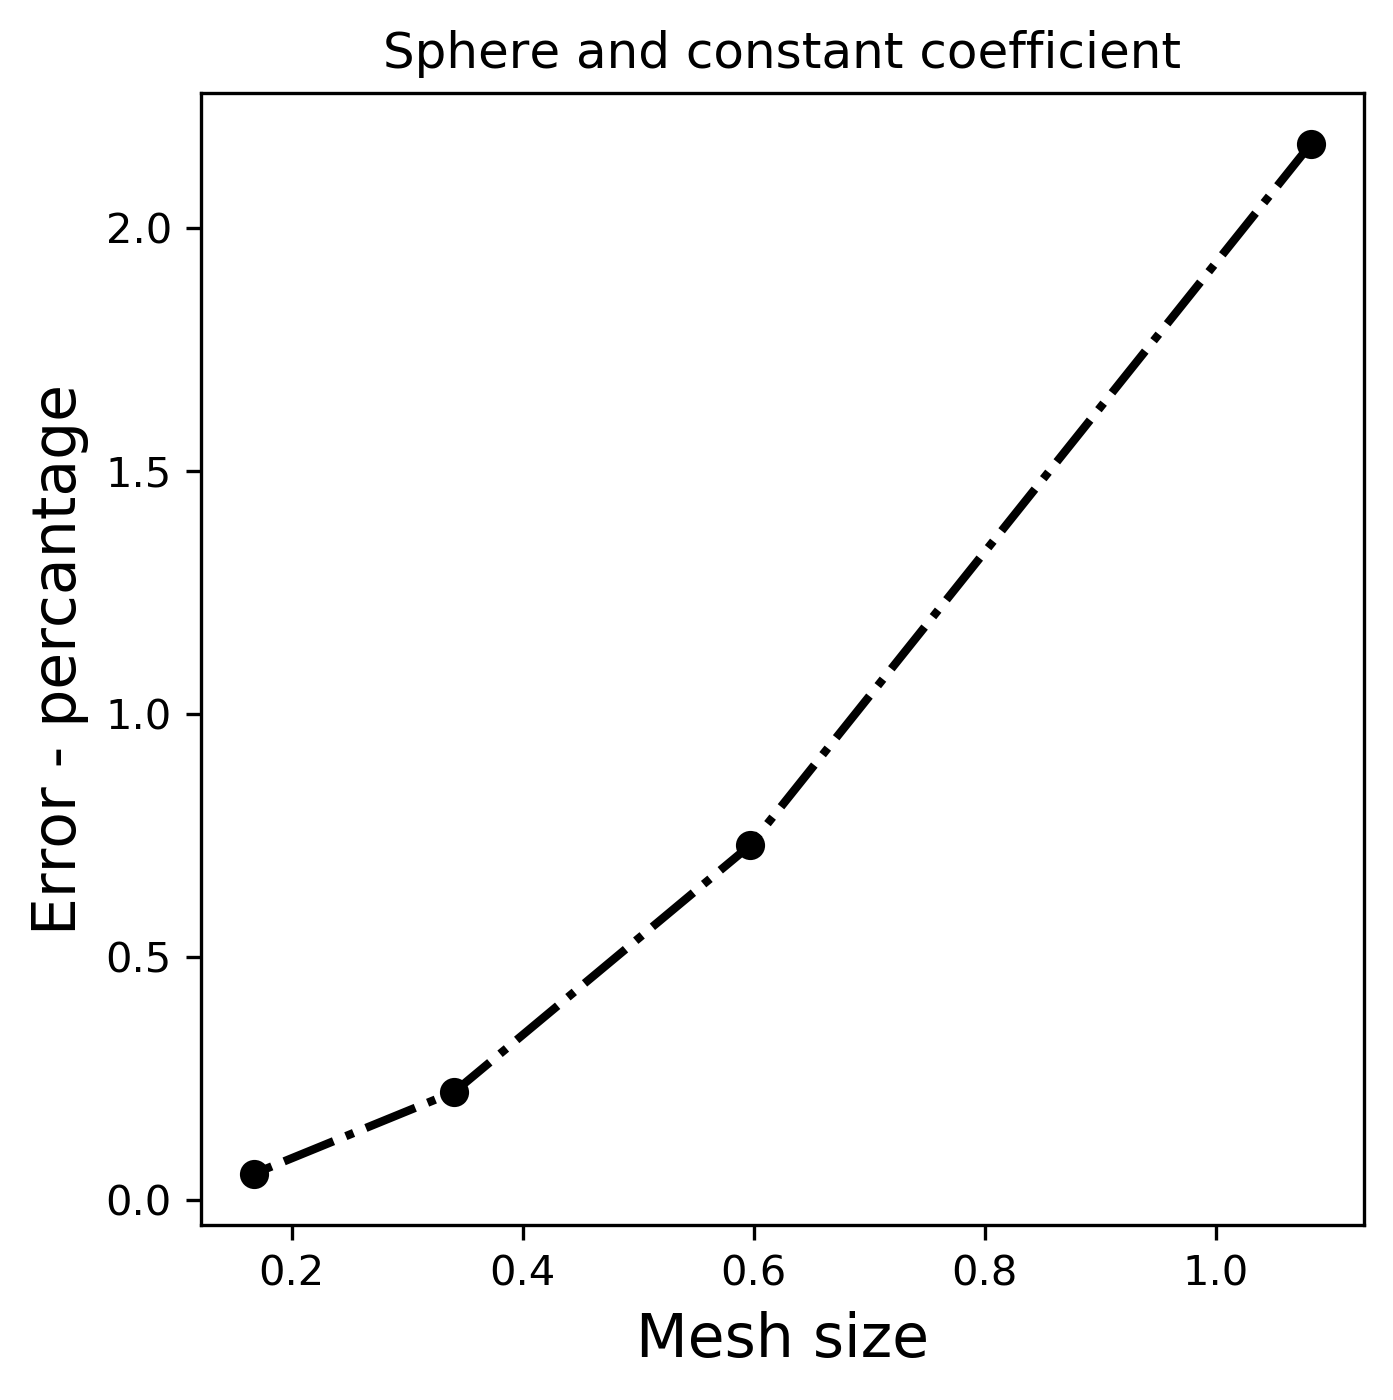
\includegraphics[width=\linewidth]{BEM_BEM_Sphere_const_coeff_error.png}
%  \caption{Error}
%\endminipage\hfill
%\minipage{0.32\textwidth}
%  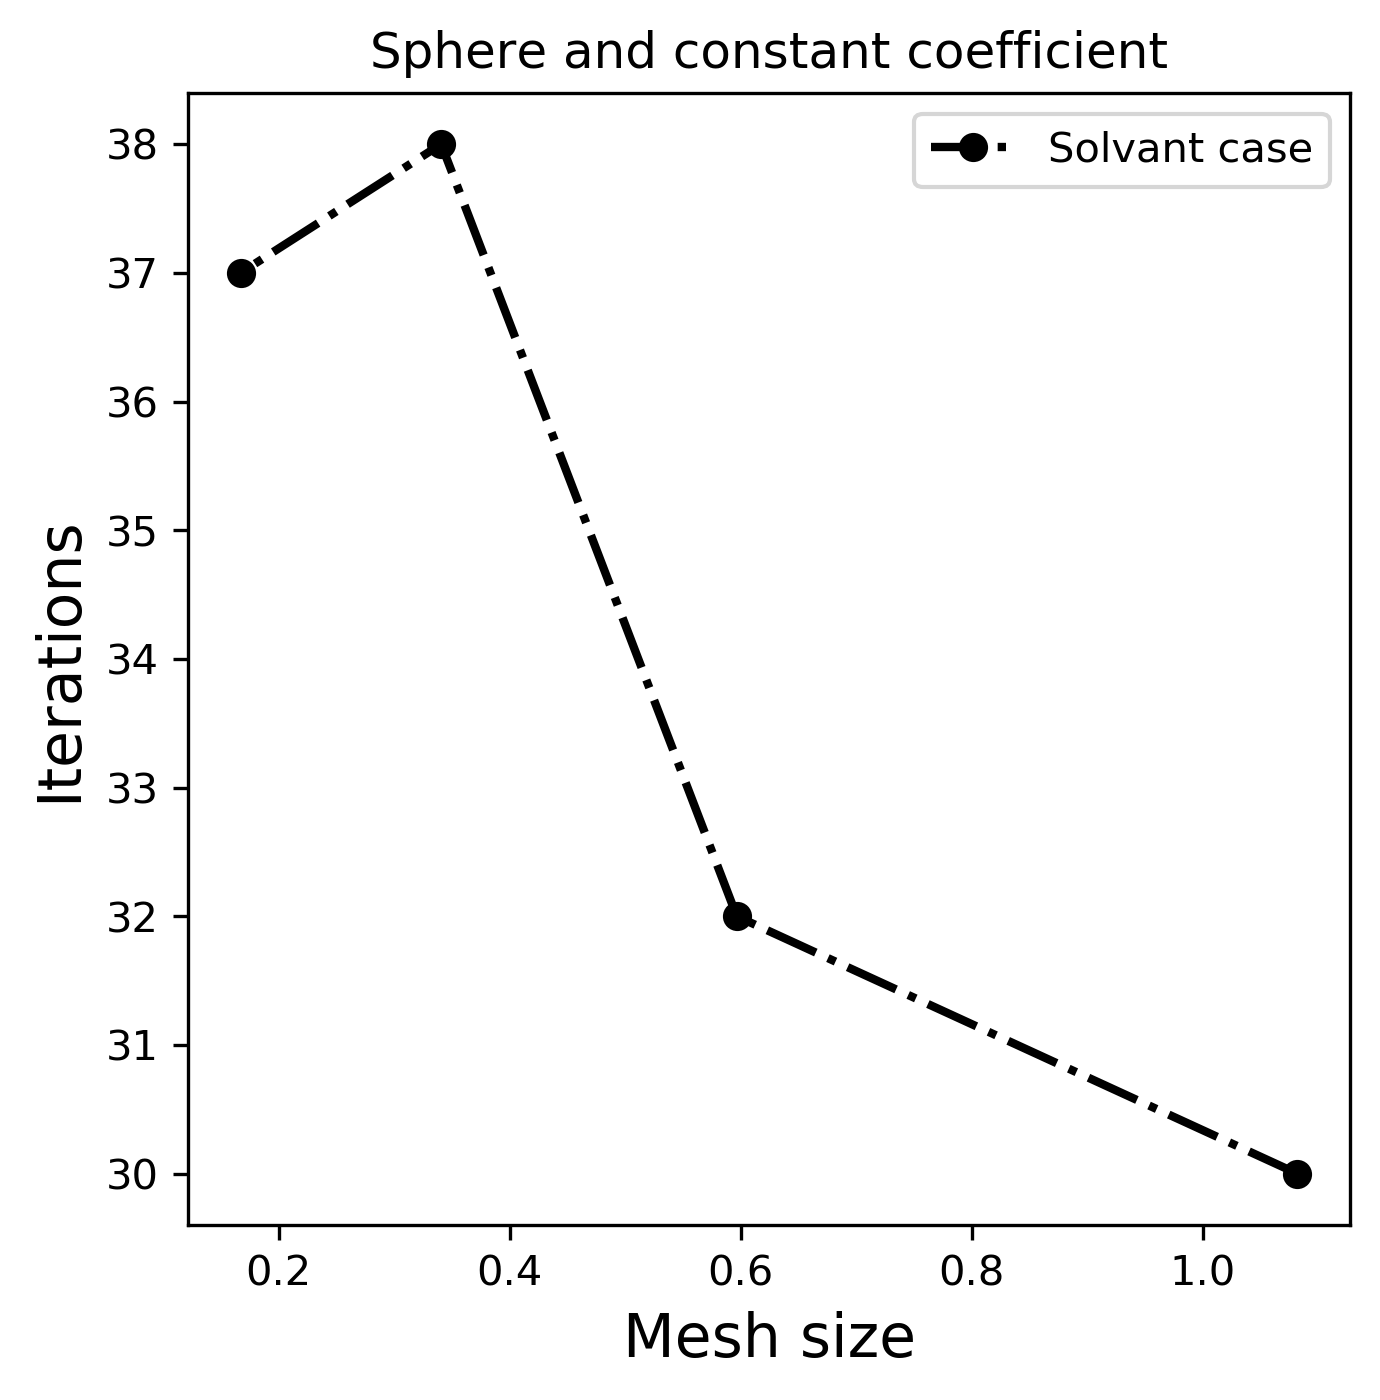
\includegraphics[width=\linewidth]{BEM_BEM_Sphere_const_coeff_iter.png}
%  \caption{Iterations}
%\endminipage\hfill
%\minipage{0.32\textwidth}%
%  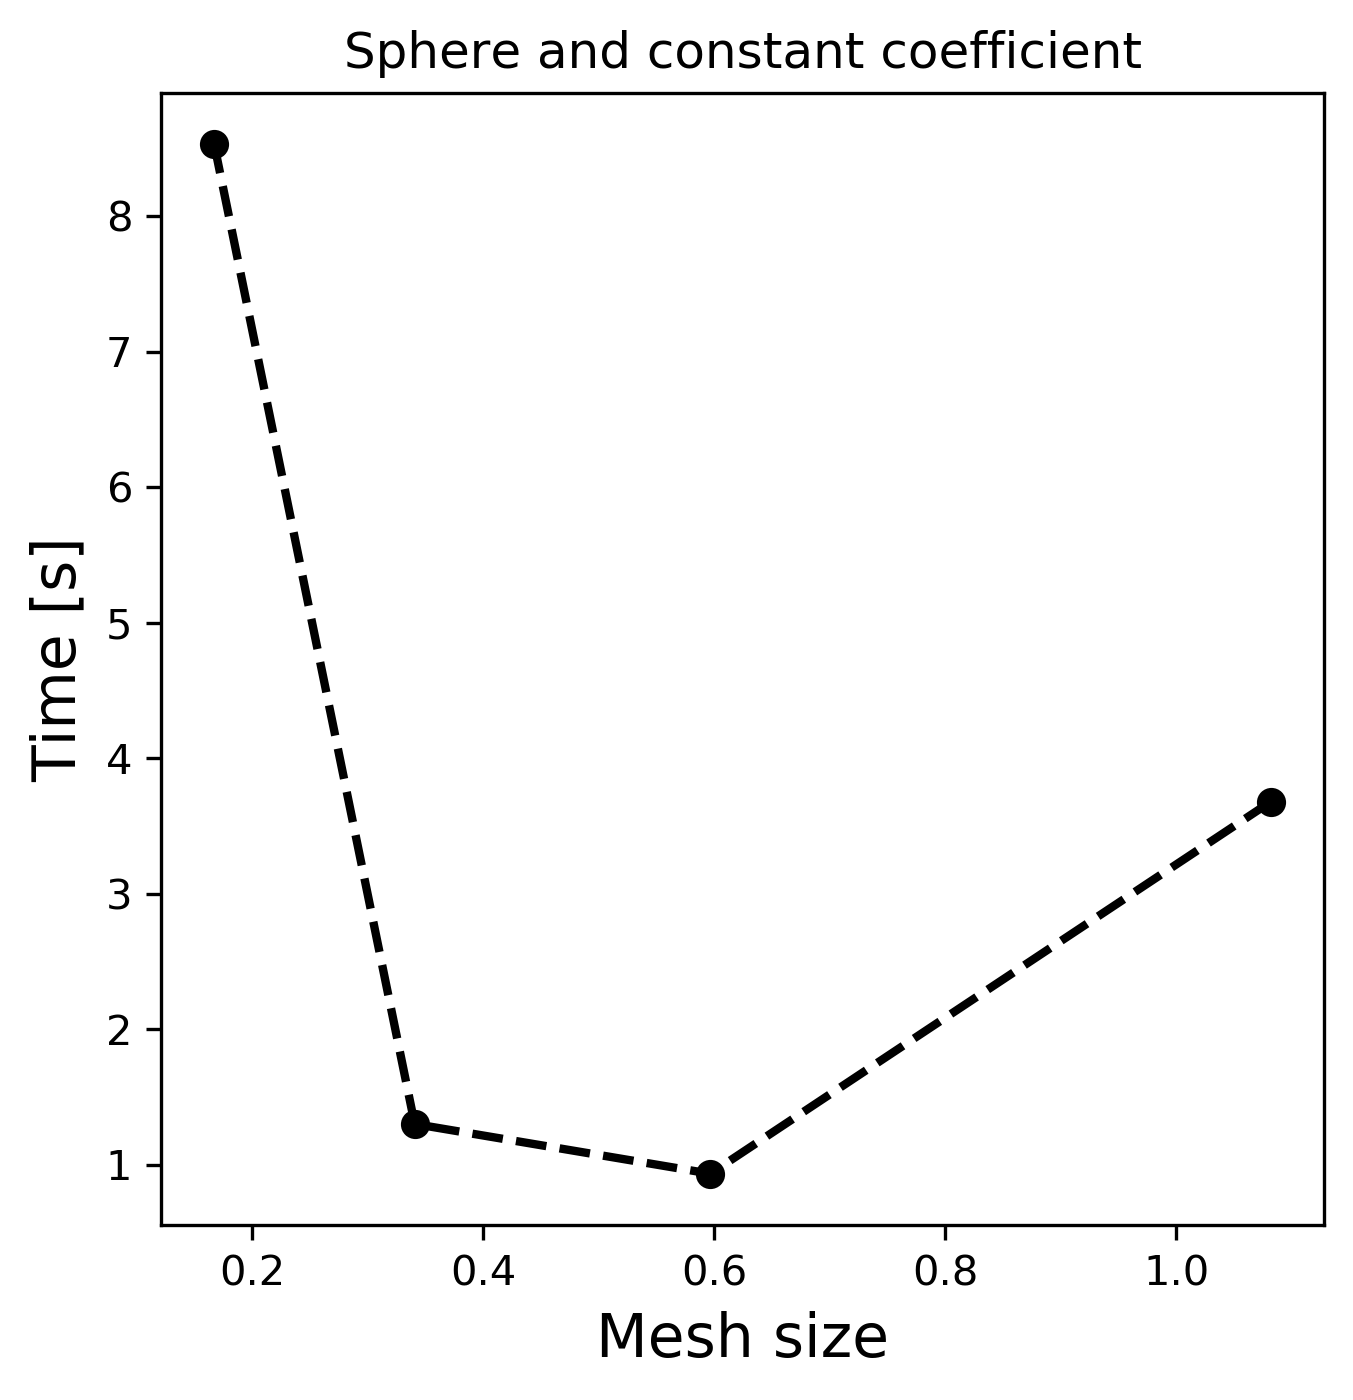
\includegraphics[width=\linewidth]{BEM_BEM_Sphere_const_coeff_time.png}
%  \caption{Computational time}
%\endminipage
%\end{figure}
%        \item Standard FEM-BEM
%\begin{figure}[!htb]
%\minipage{0.32\textwidth}
%  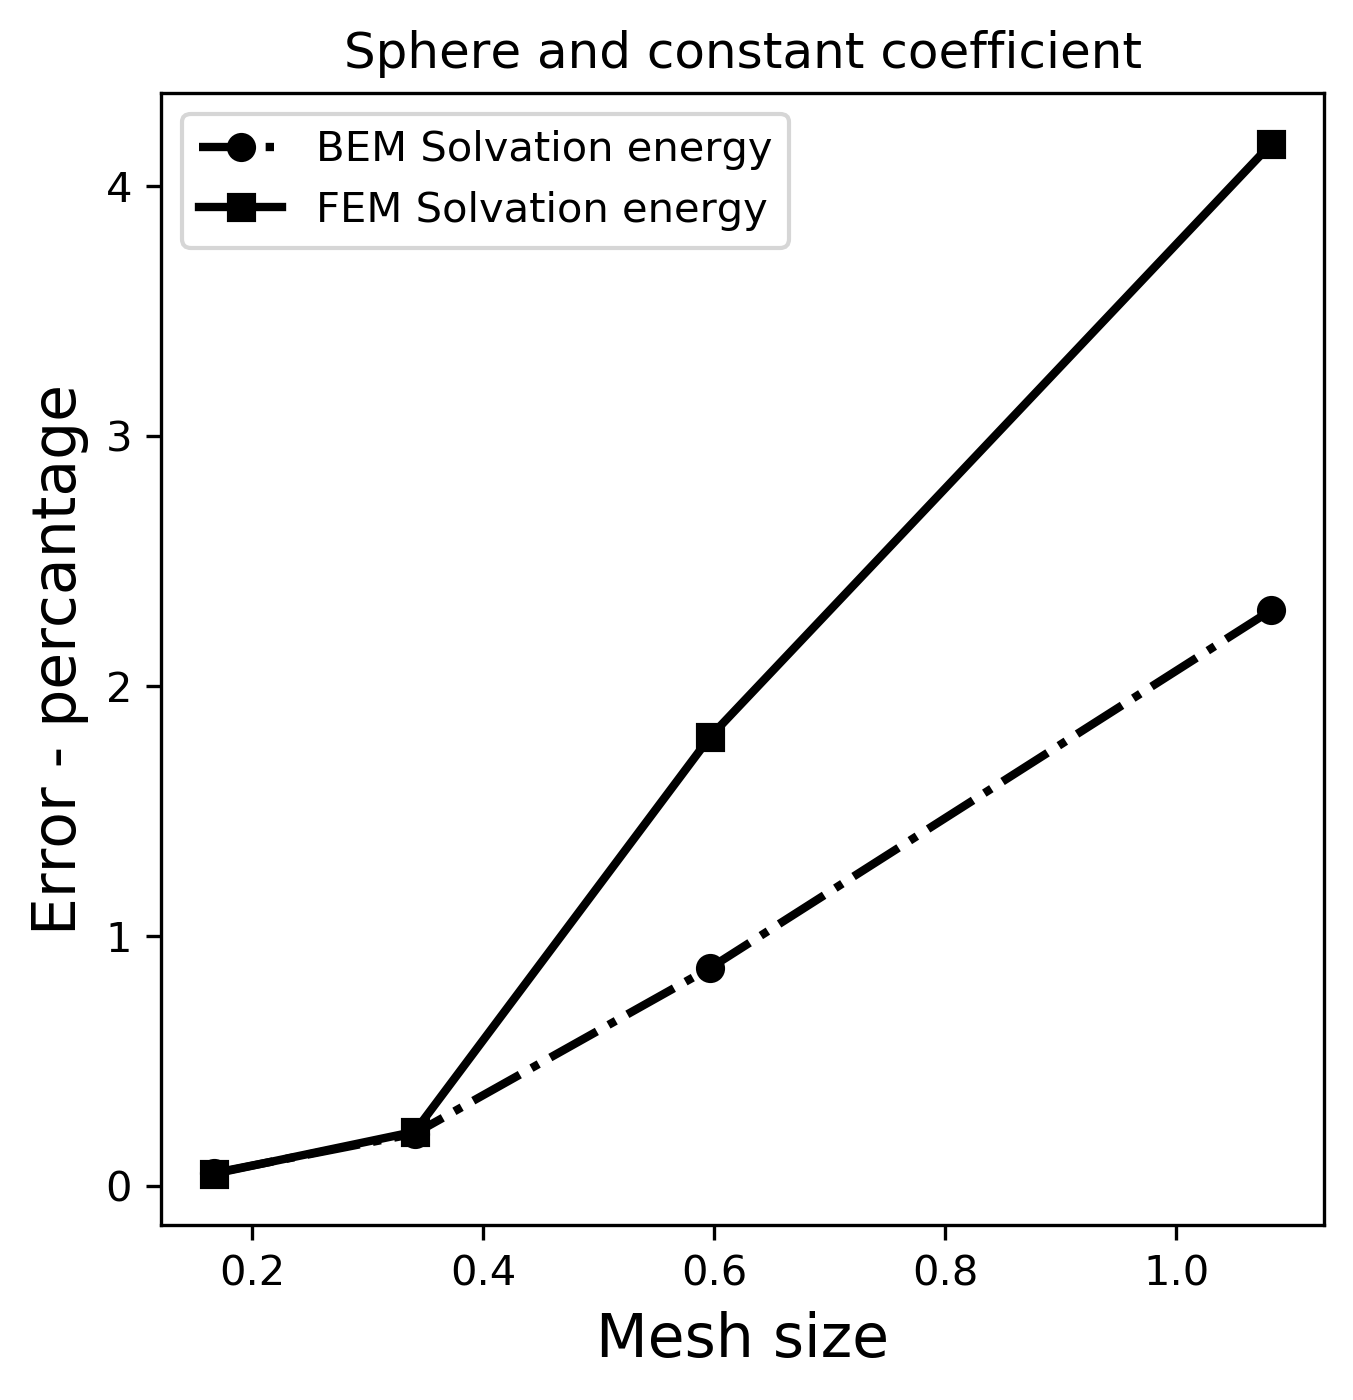
\includegraphics[width=\linewidth]{FEM_BEM_Sphere_const_coeff_error.png}
%  \caption{Error}
%\endminipage\hfill
%\minipage{0.32\textwidth}
%  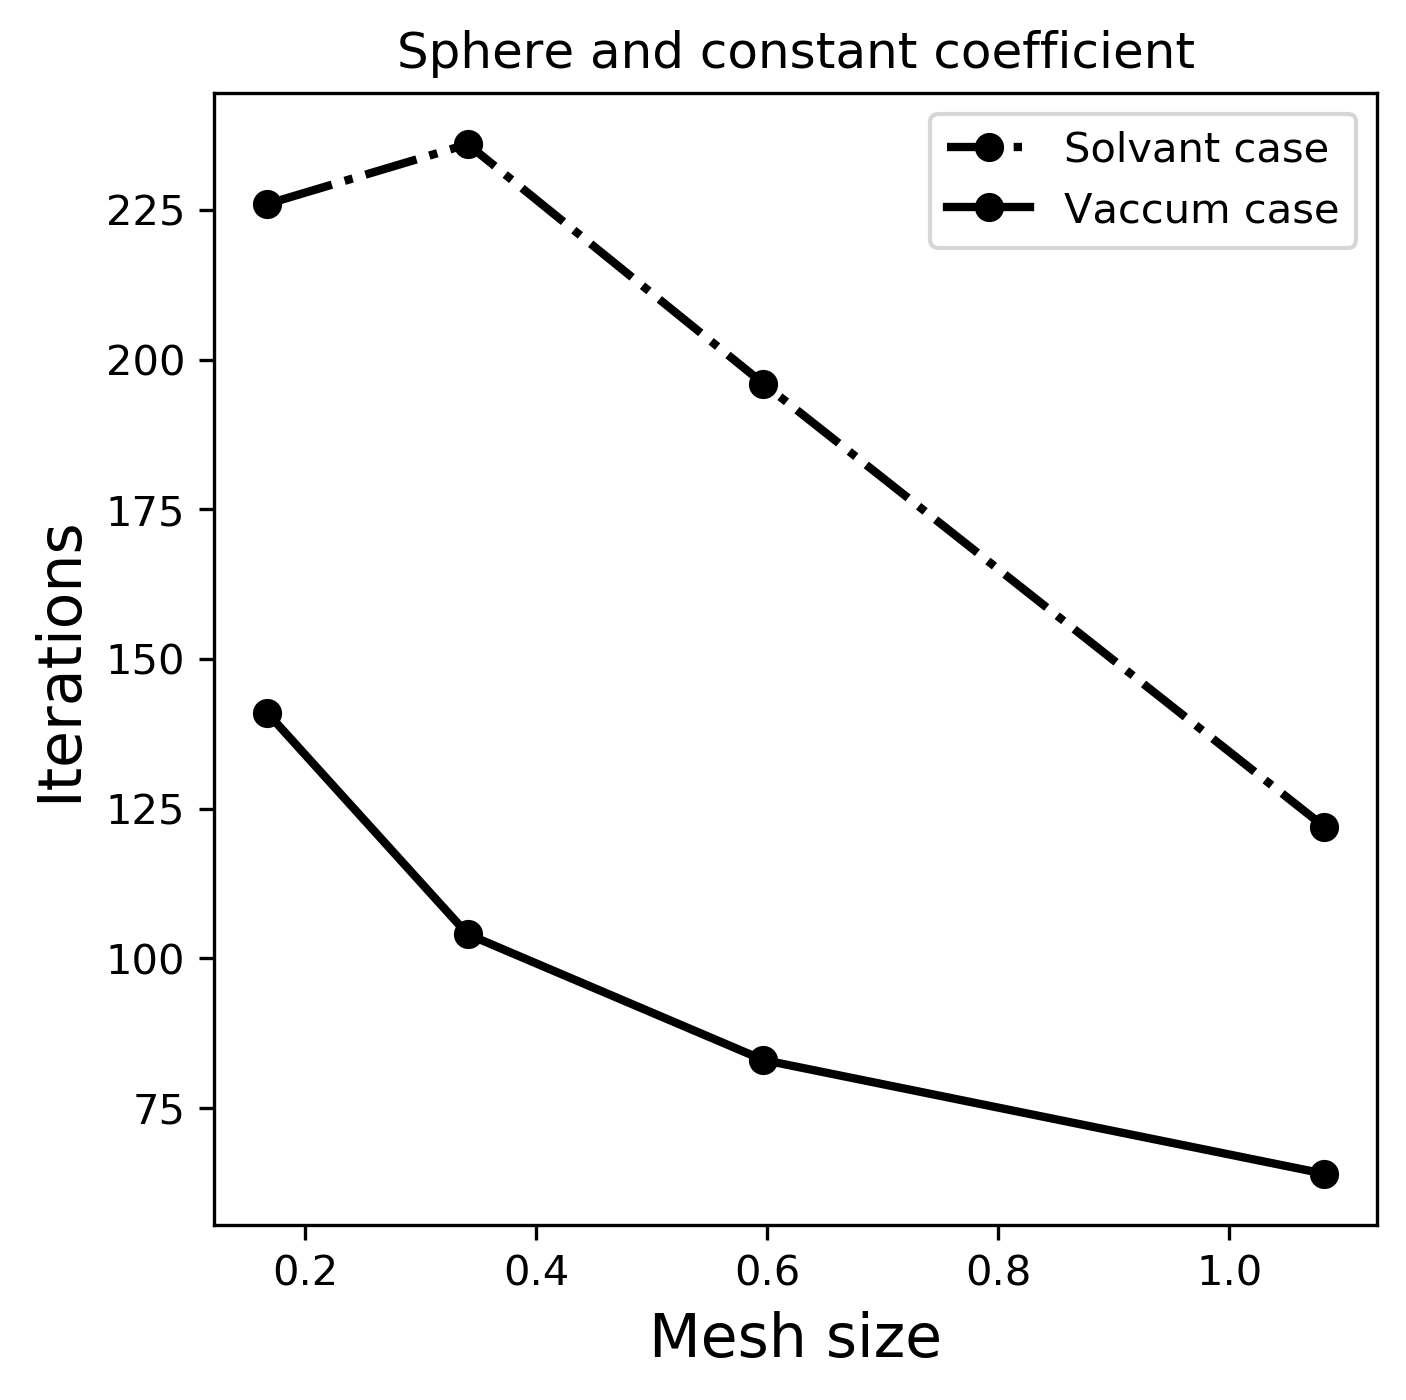
\includegraphics[width=\linewidth]{FEM_BEM_Sphere_const_coeff_iter.png}
%  \caption{Iterations}
%\endminipage\hfill
%\minipage{0.32\textwidth}%
%  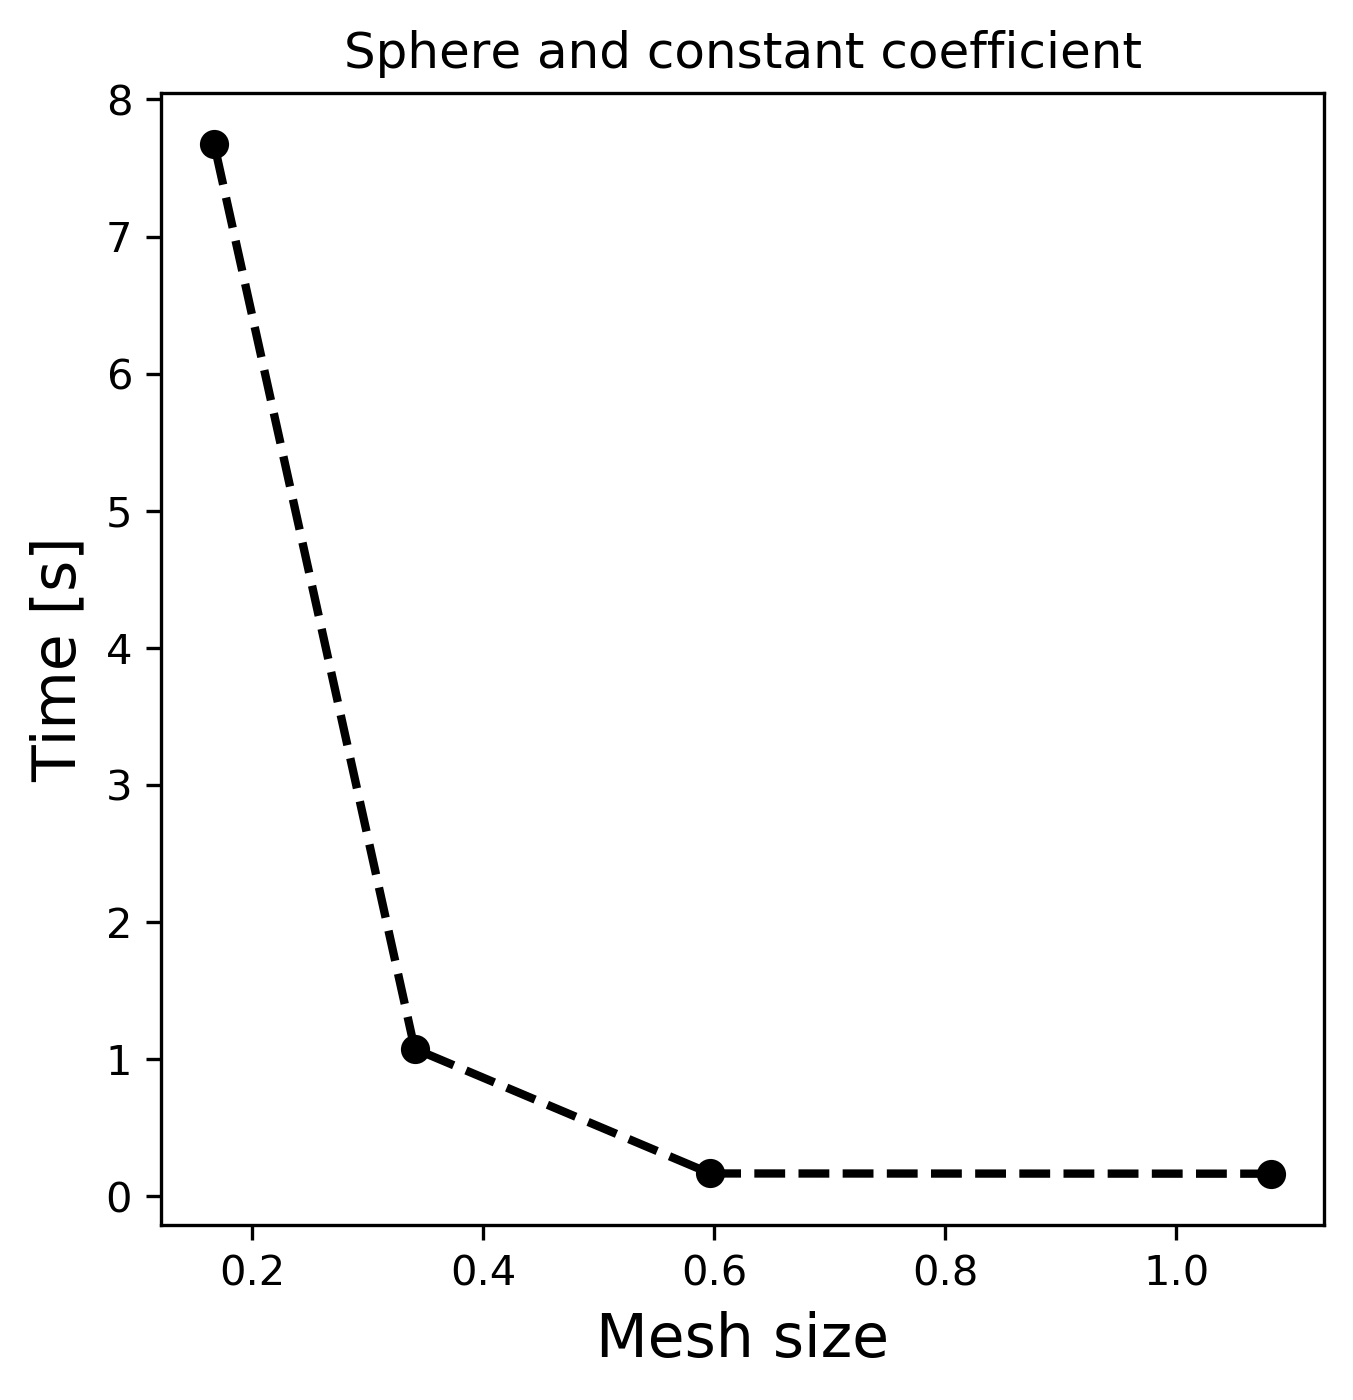
\includegraphics[width=\linewidth]{FEM_BEM_Sphere_const_coeff_time.png}
%  \caption{Computational time}
%\endminipage
%\end{figure}
%        \item Hybrid FEM-BEM
%\begin{figure}[!htb]
%\minipage{0.32\textwidth}
%  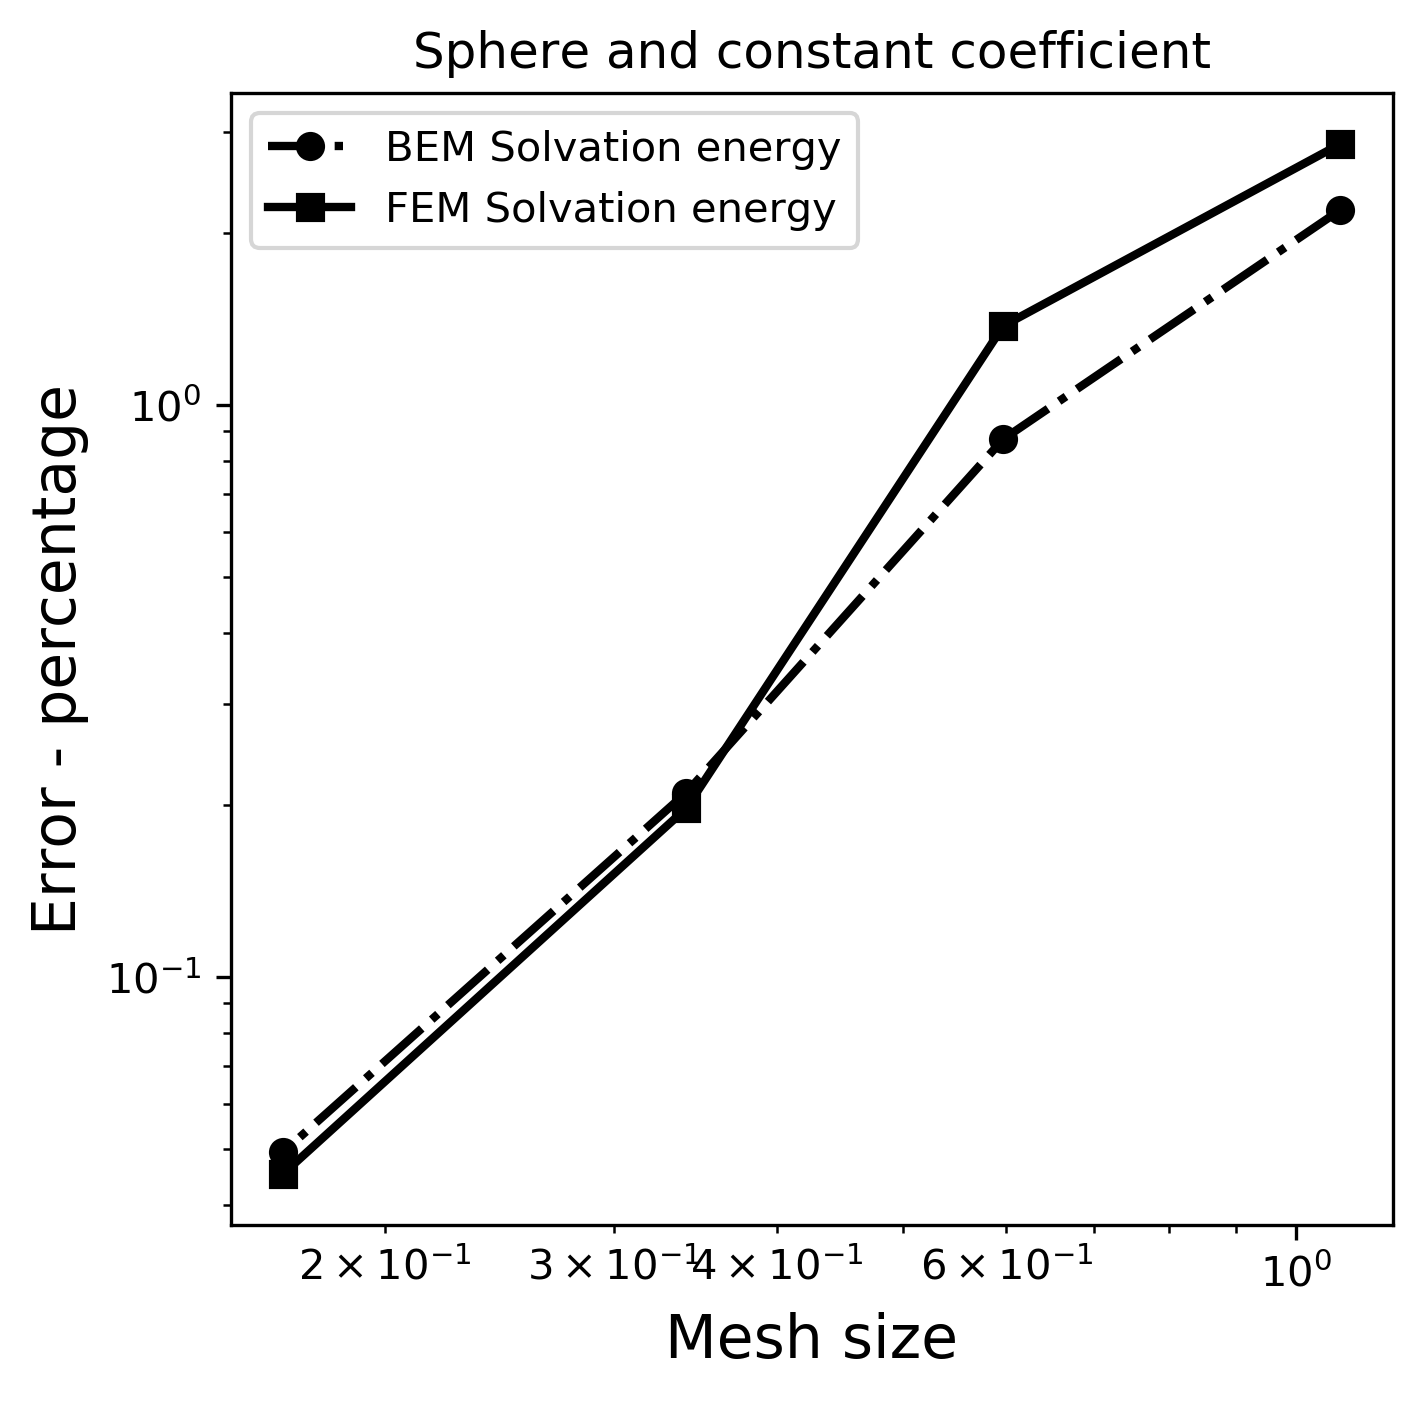
\includegraphics[width=\linewidth]{Hybrid_FEM_BEM_Sphere_const_coeff_error.png}
%  \caption{Error}
%\endminipage\hfill
%\minipage{0.32\textwidth}
%  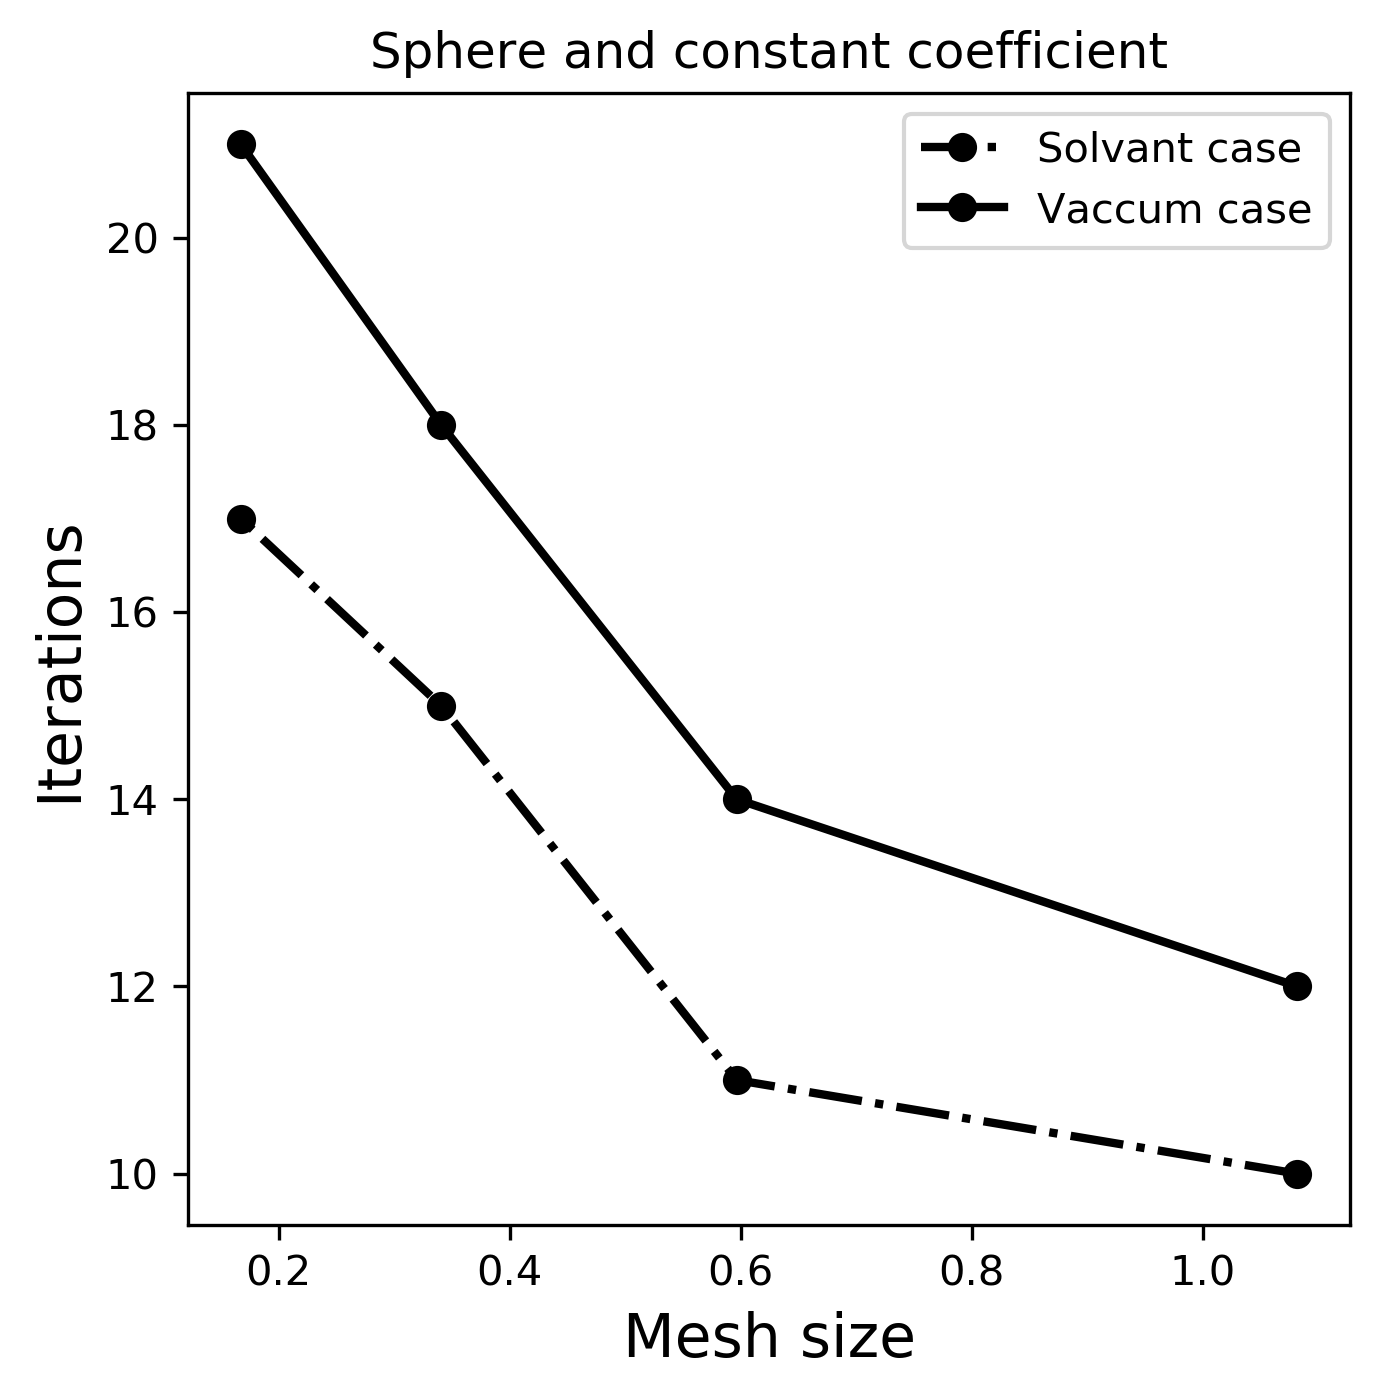
\includegraphics[width=\linewidth]{Hybrid_FEM_BEM_Sphere_const_coeff_iter.png}
%  \caption{Iterations}
%\endminipage\hfill
%\minipage{0.32\textwidth}%
%  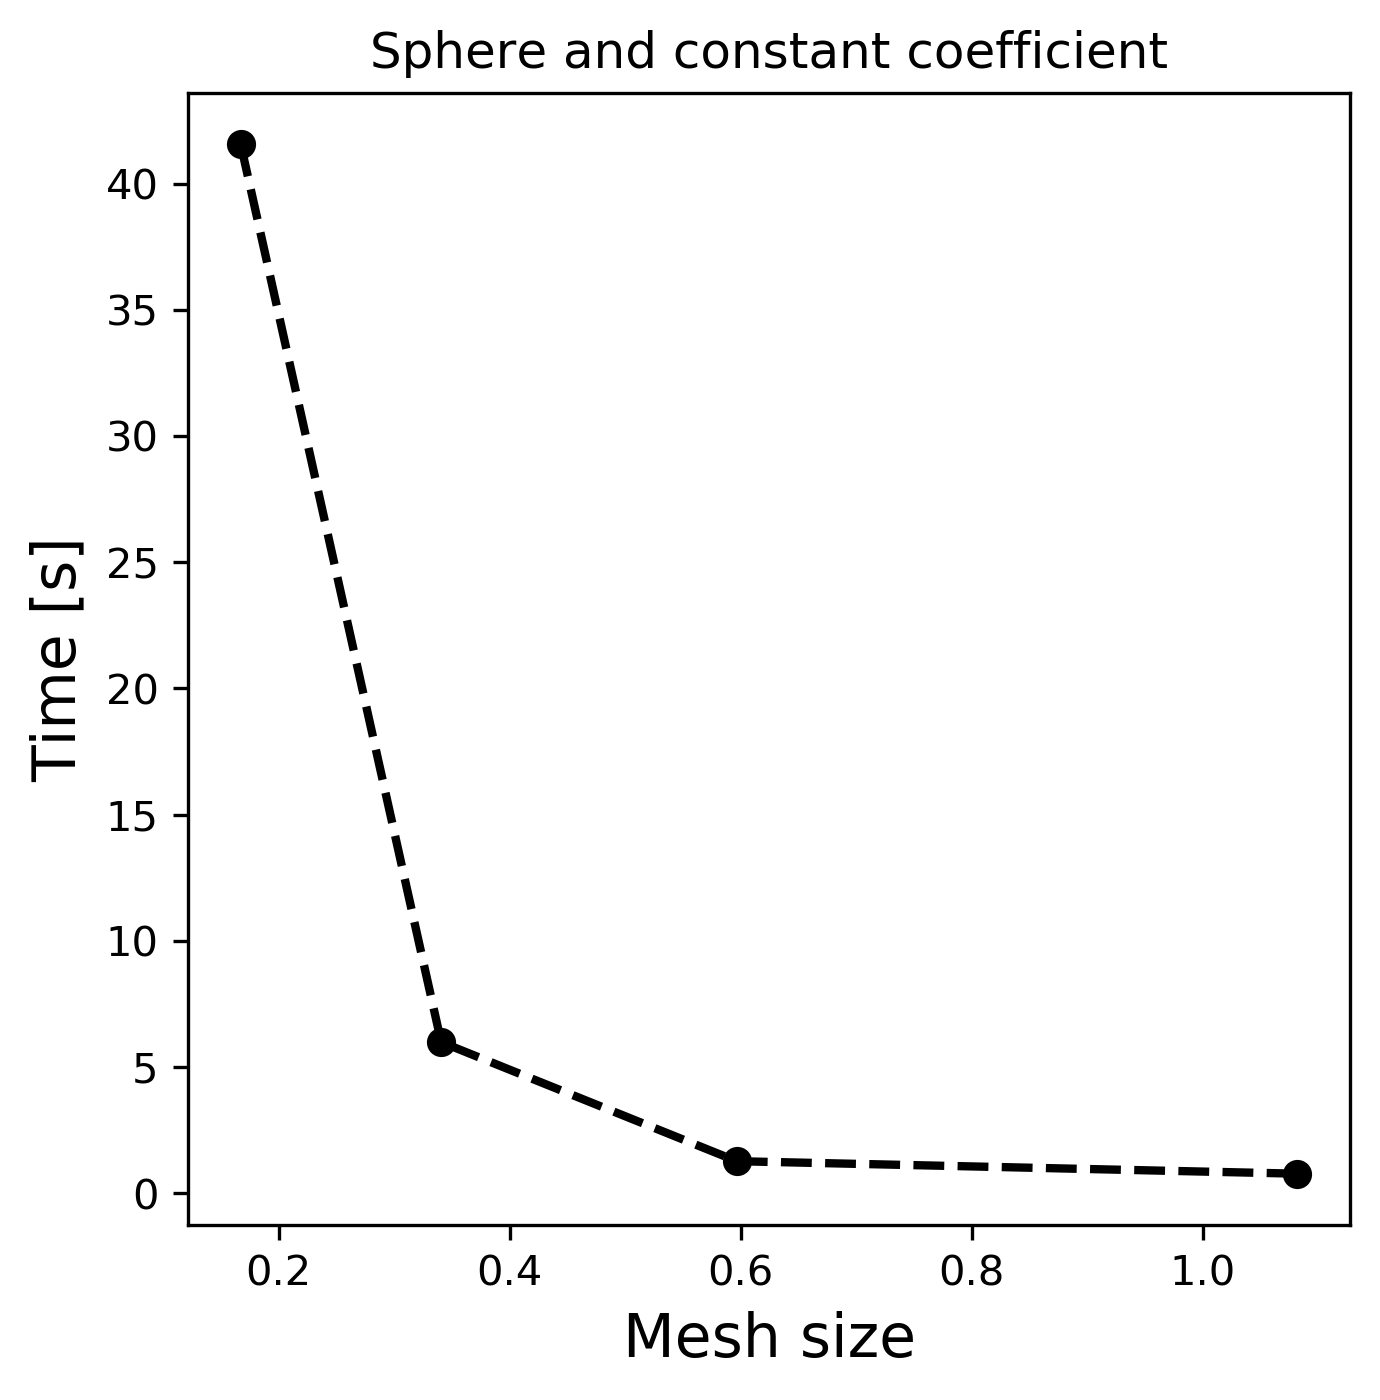
\includegraphics[width=\linewidth]{Hybrid_FEM_BEM_Sphere_const_coeff_time.png}
%  \caption{Computational time}
%\endminipage
%\end{figure}
%    \end{itemize}
%\end{itemize}

\subsection*{\sffamily \large Performance for a molecular geometry}
\begin{itemize}
    \item Use arginine or a small protein (1PGB?)
    \begin{itemize}
        \item BEM-BEM
\begin{figure}[!htb]
\minipage{0.45\textwidth}
  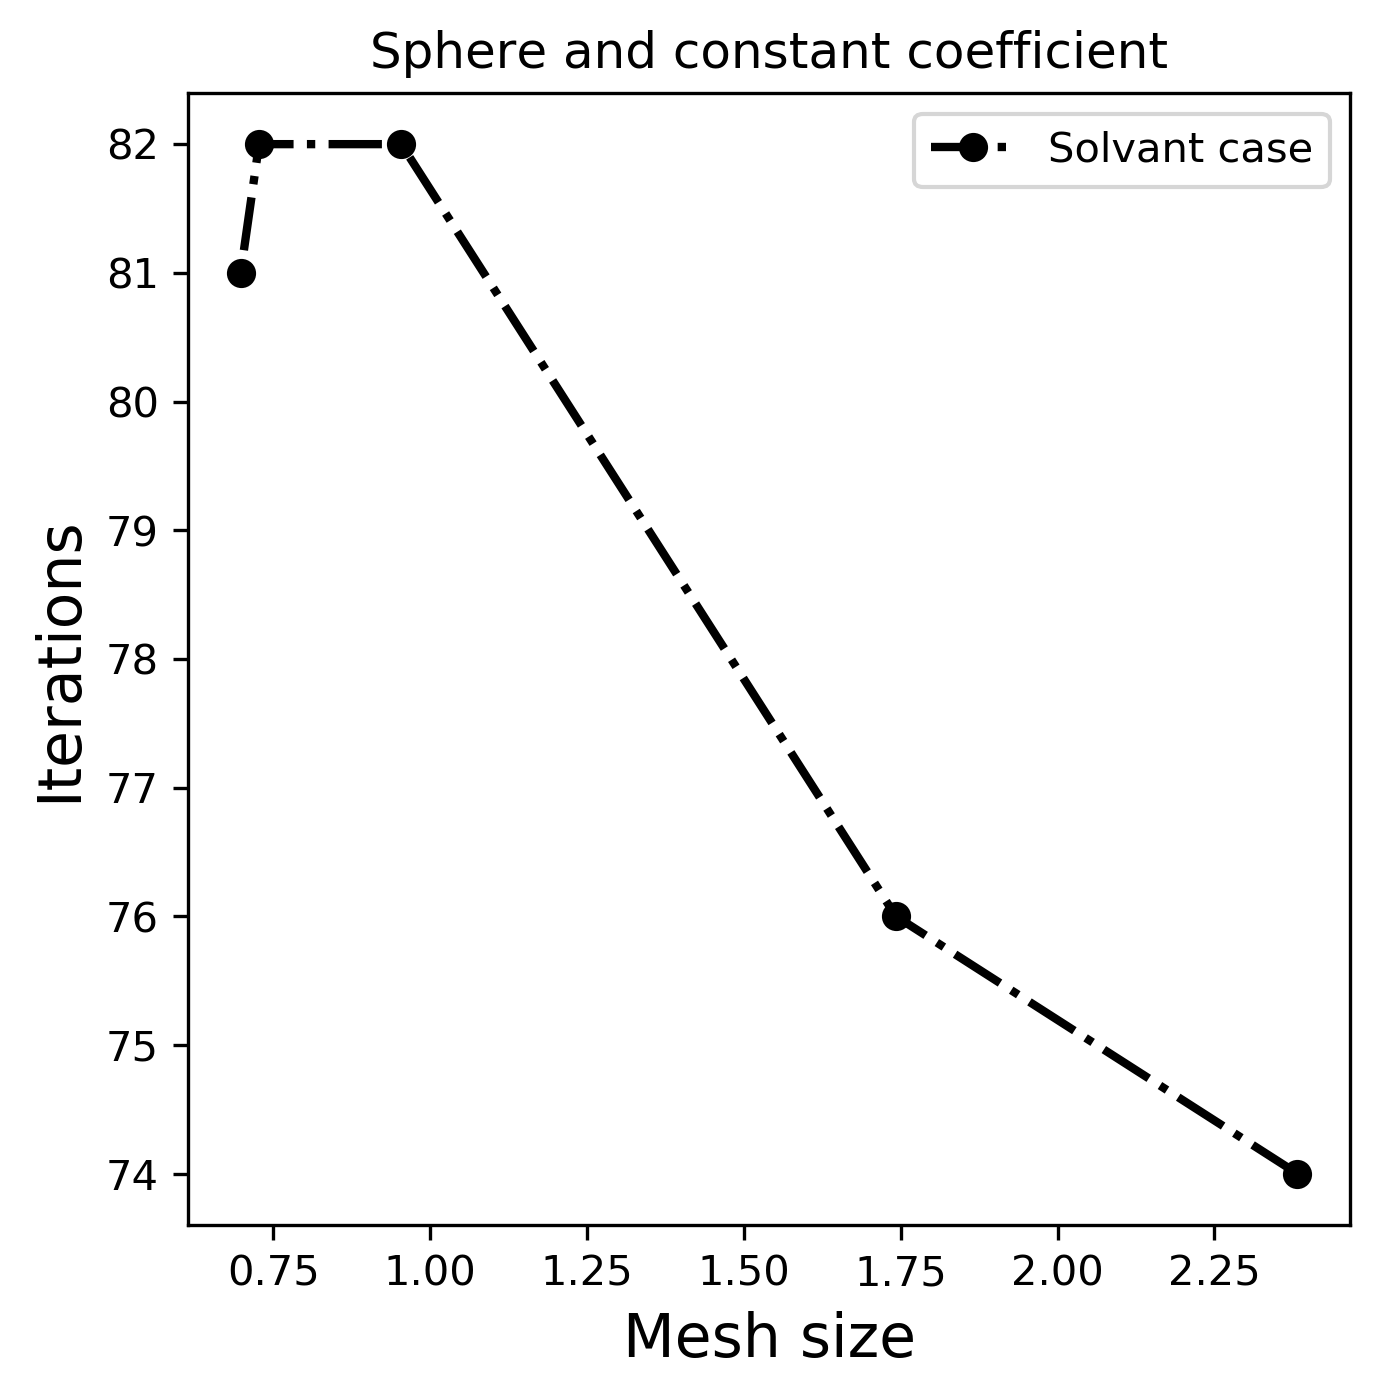
\includegraphics[width=\linewidth]{BEM_BEM_Arginine_const_coeff_iter.png}
  \caption{Iterations}
\endminipage\hfill
\minipage{0.45\textwidth}%
  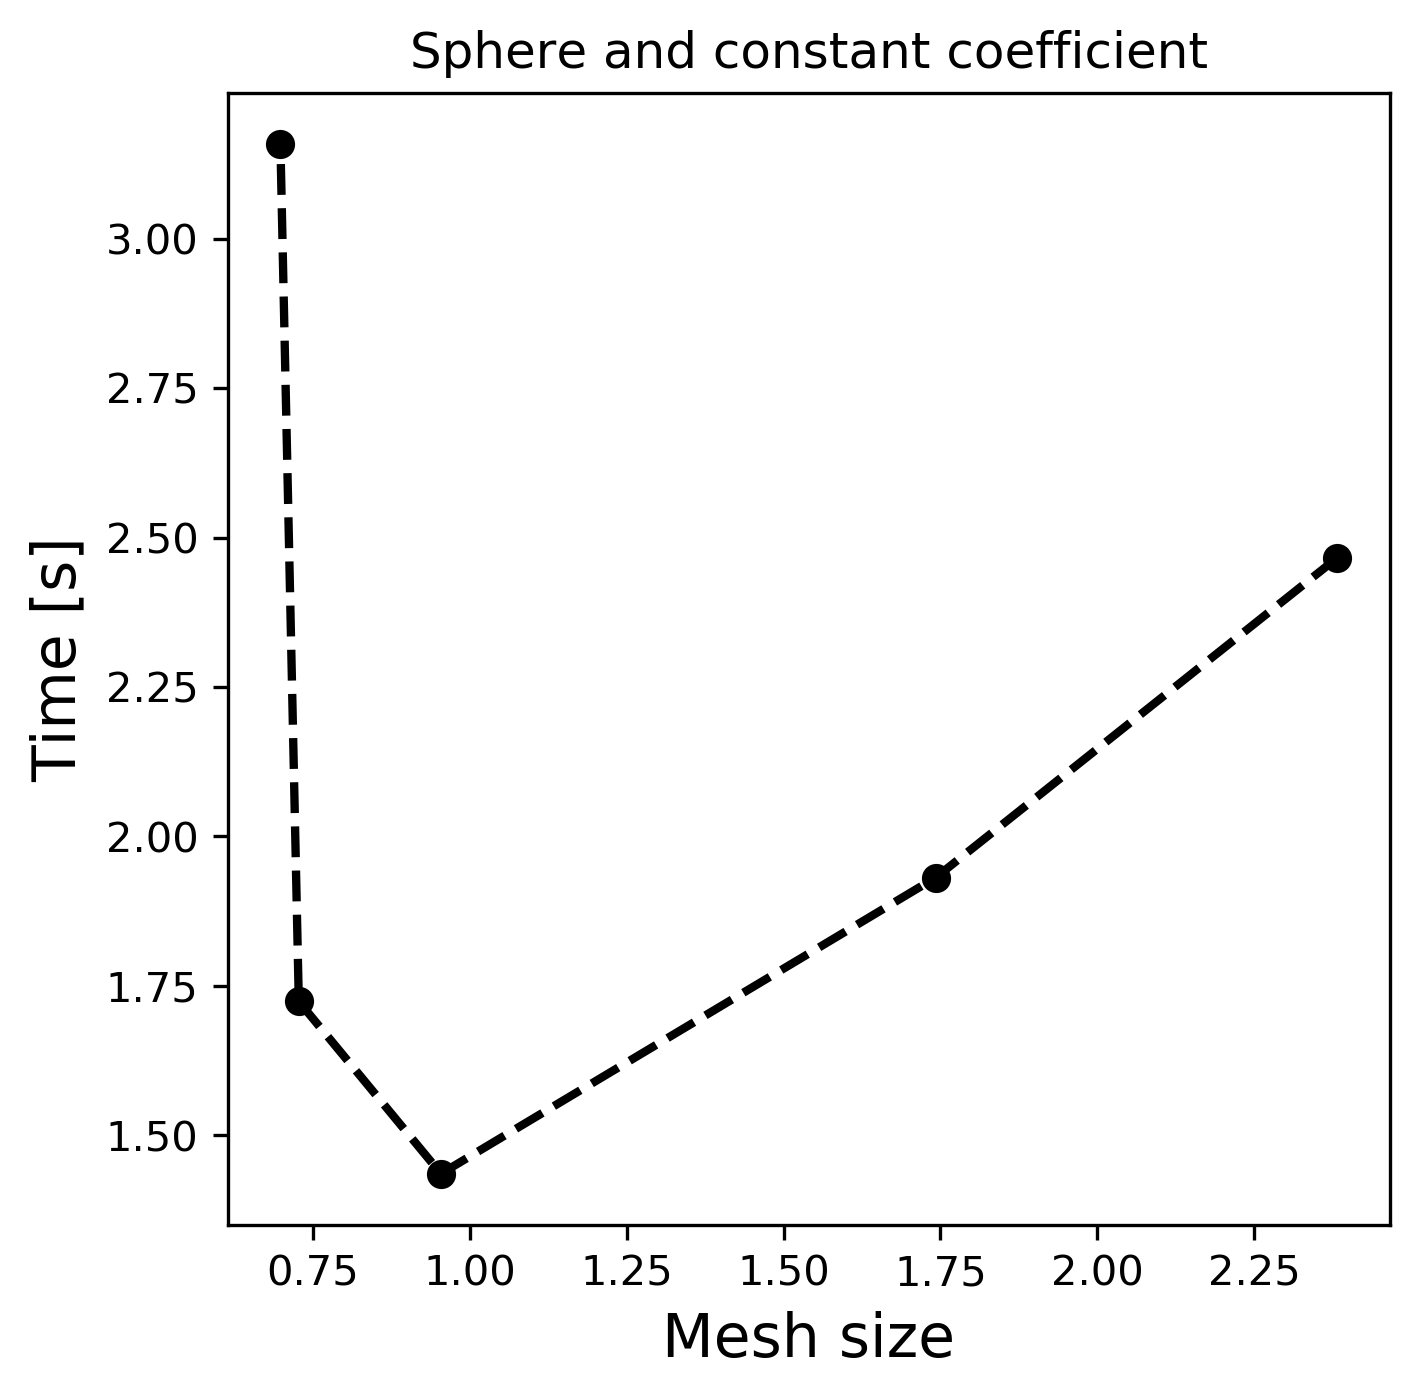
\includegraphics[width=\linewidth]{BEM_BEM_Arginine_const_coeff_time.png}
  \caption{Computational time}
\endminipage
\end{figure}
        \item Standard FEM-BEM
\begin{figure}[!htb]
\minipage{0.45\textwidth}
  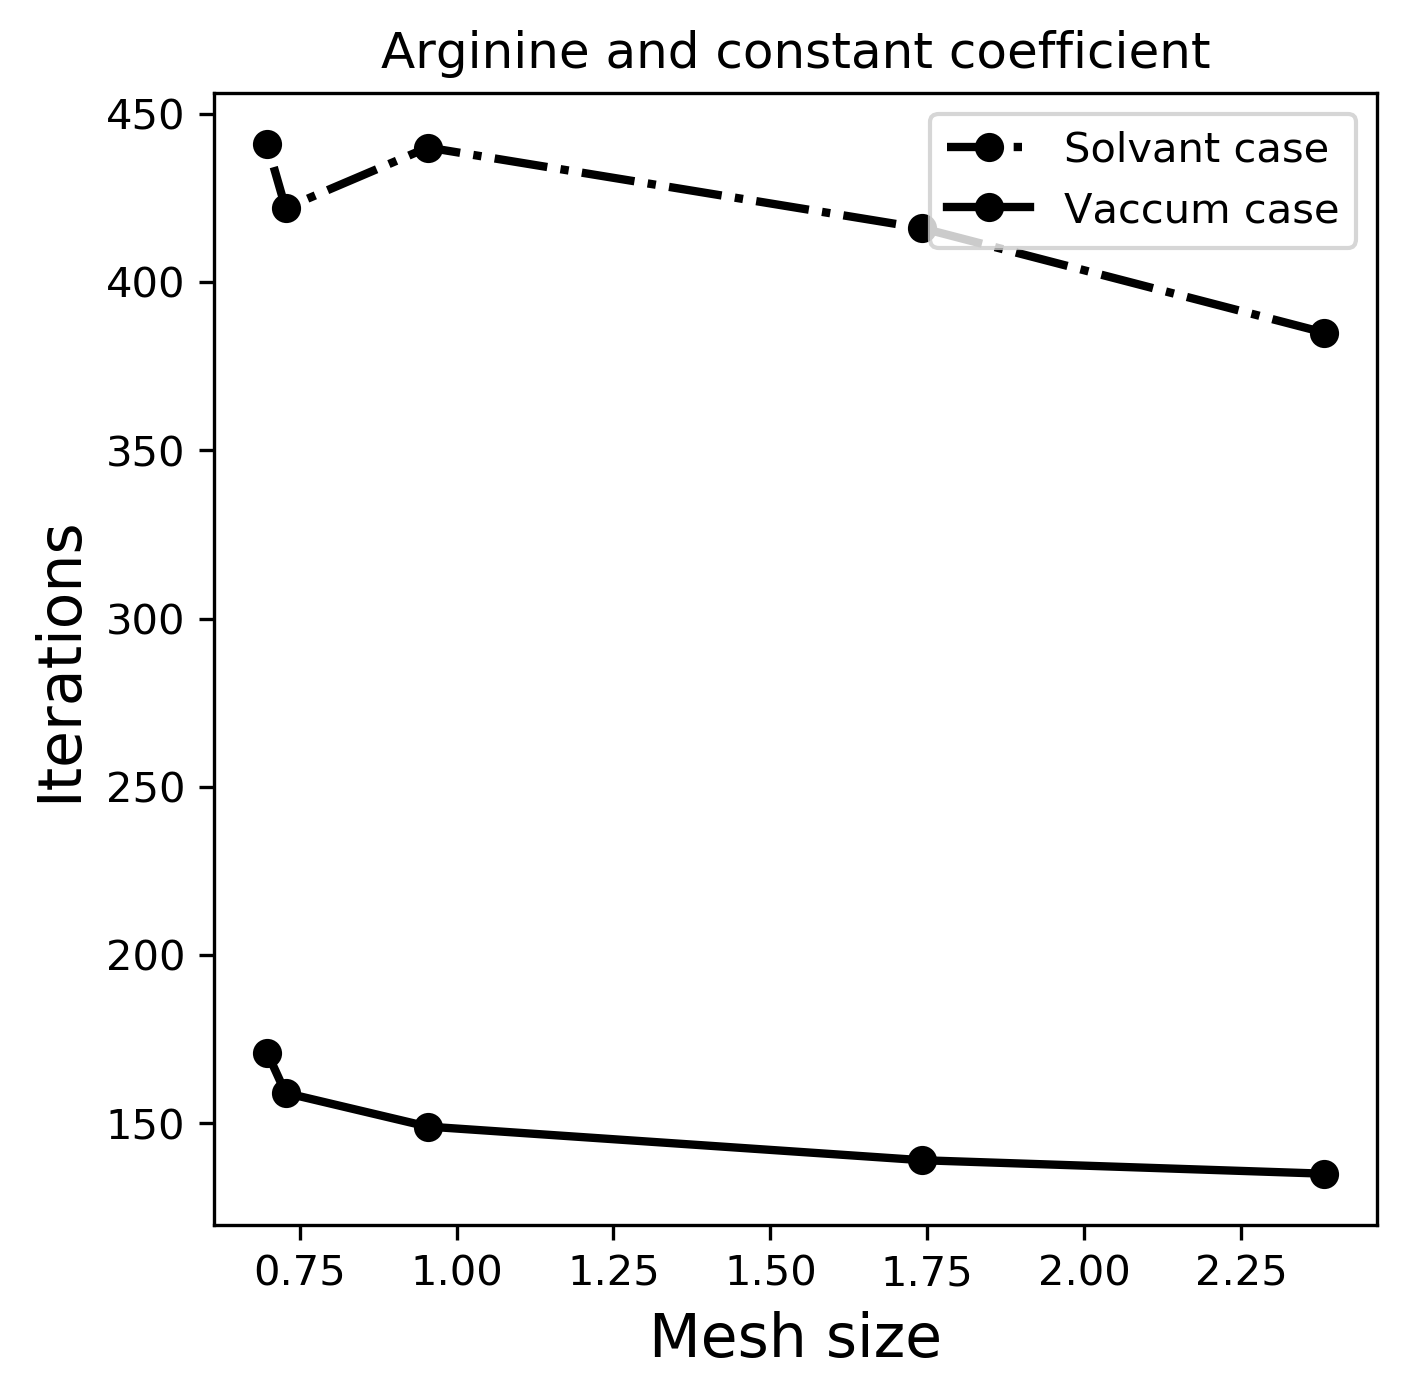
\includegraphics[width=\linewidth]{FEM_BEM_Arginine_const_coeff_iter.png}
  \caption{Iterations}
\endminipage\hfill
\minipage{0.45\textwidth}%
  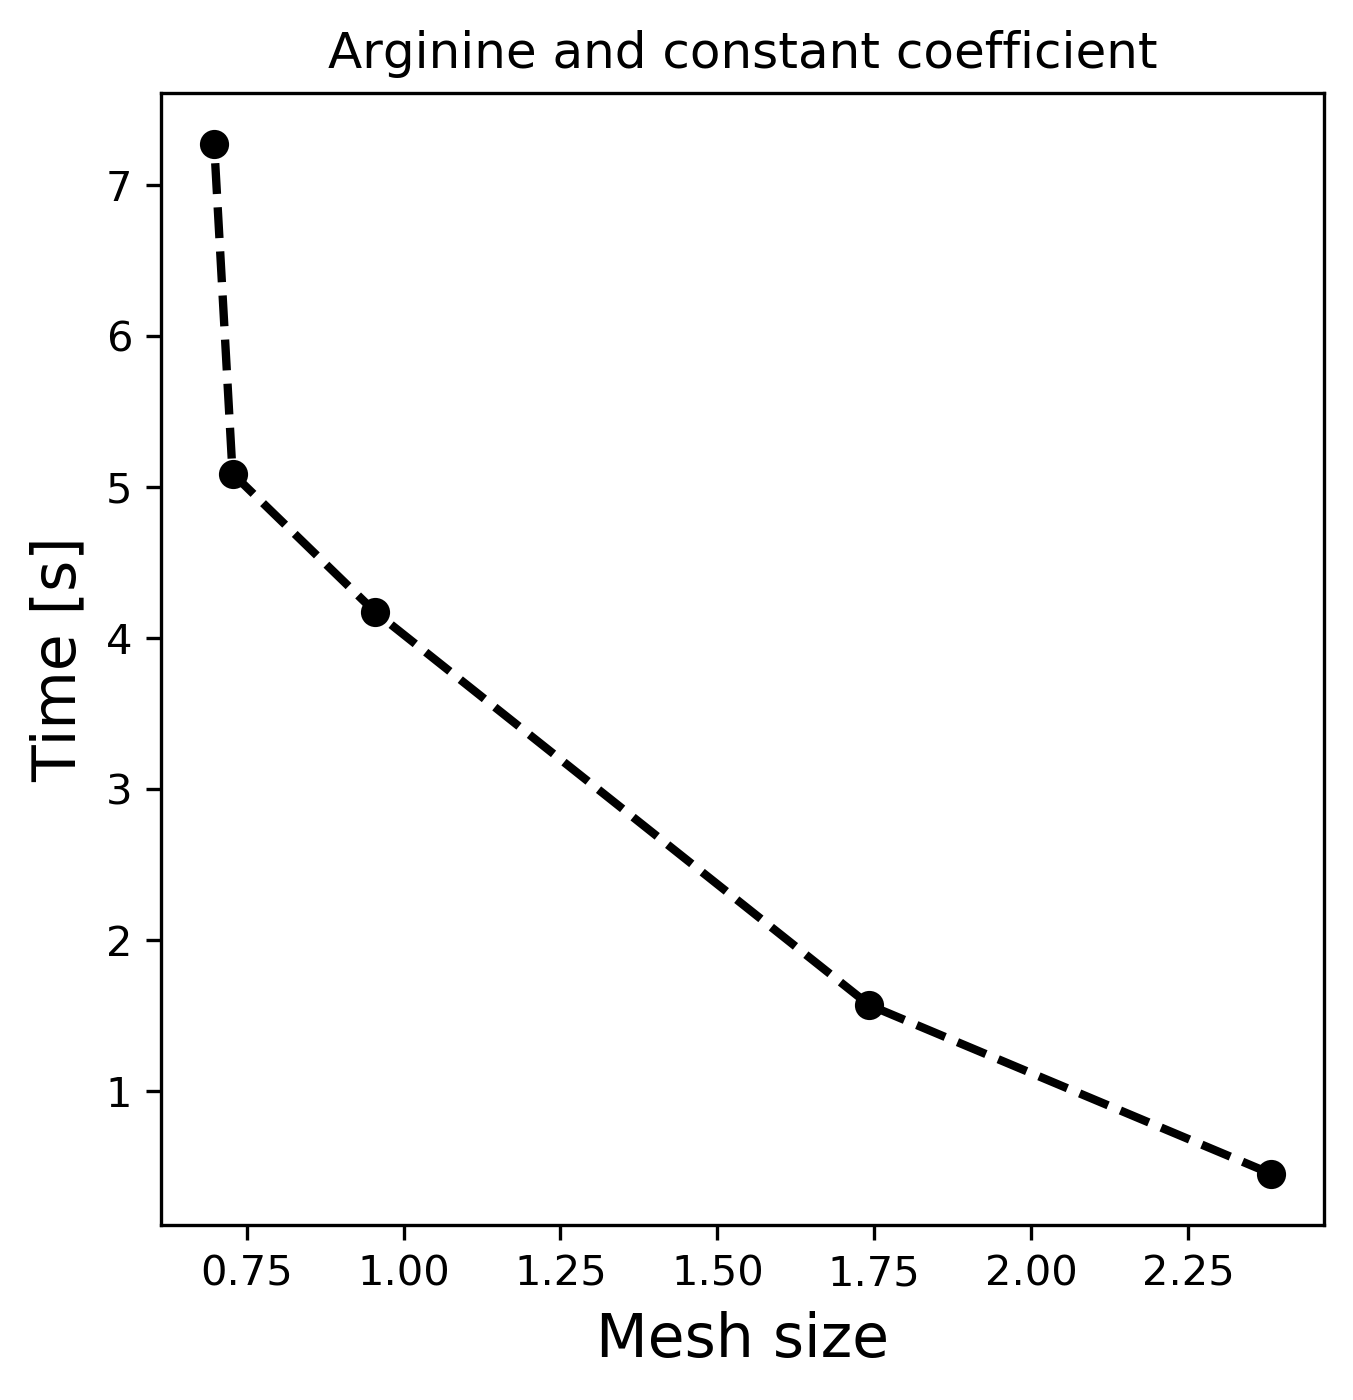
\includegraphics[width=\linewidth]{FEM_BEM_Arginine_const_coeff_time.png}
  \caption{Computational time}
\endminipage
\end{figure}
        \item Hybrid FEM-BEM
\begin{figure}[!htb]
\minipage{0.45\textwidth}
  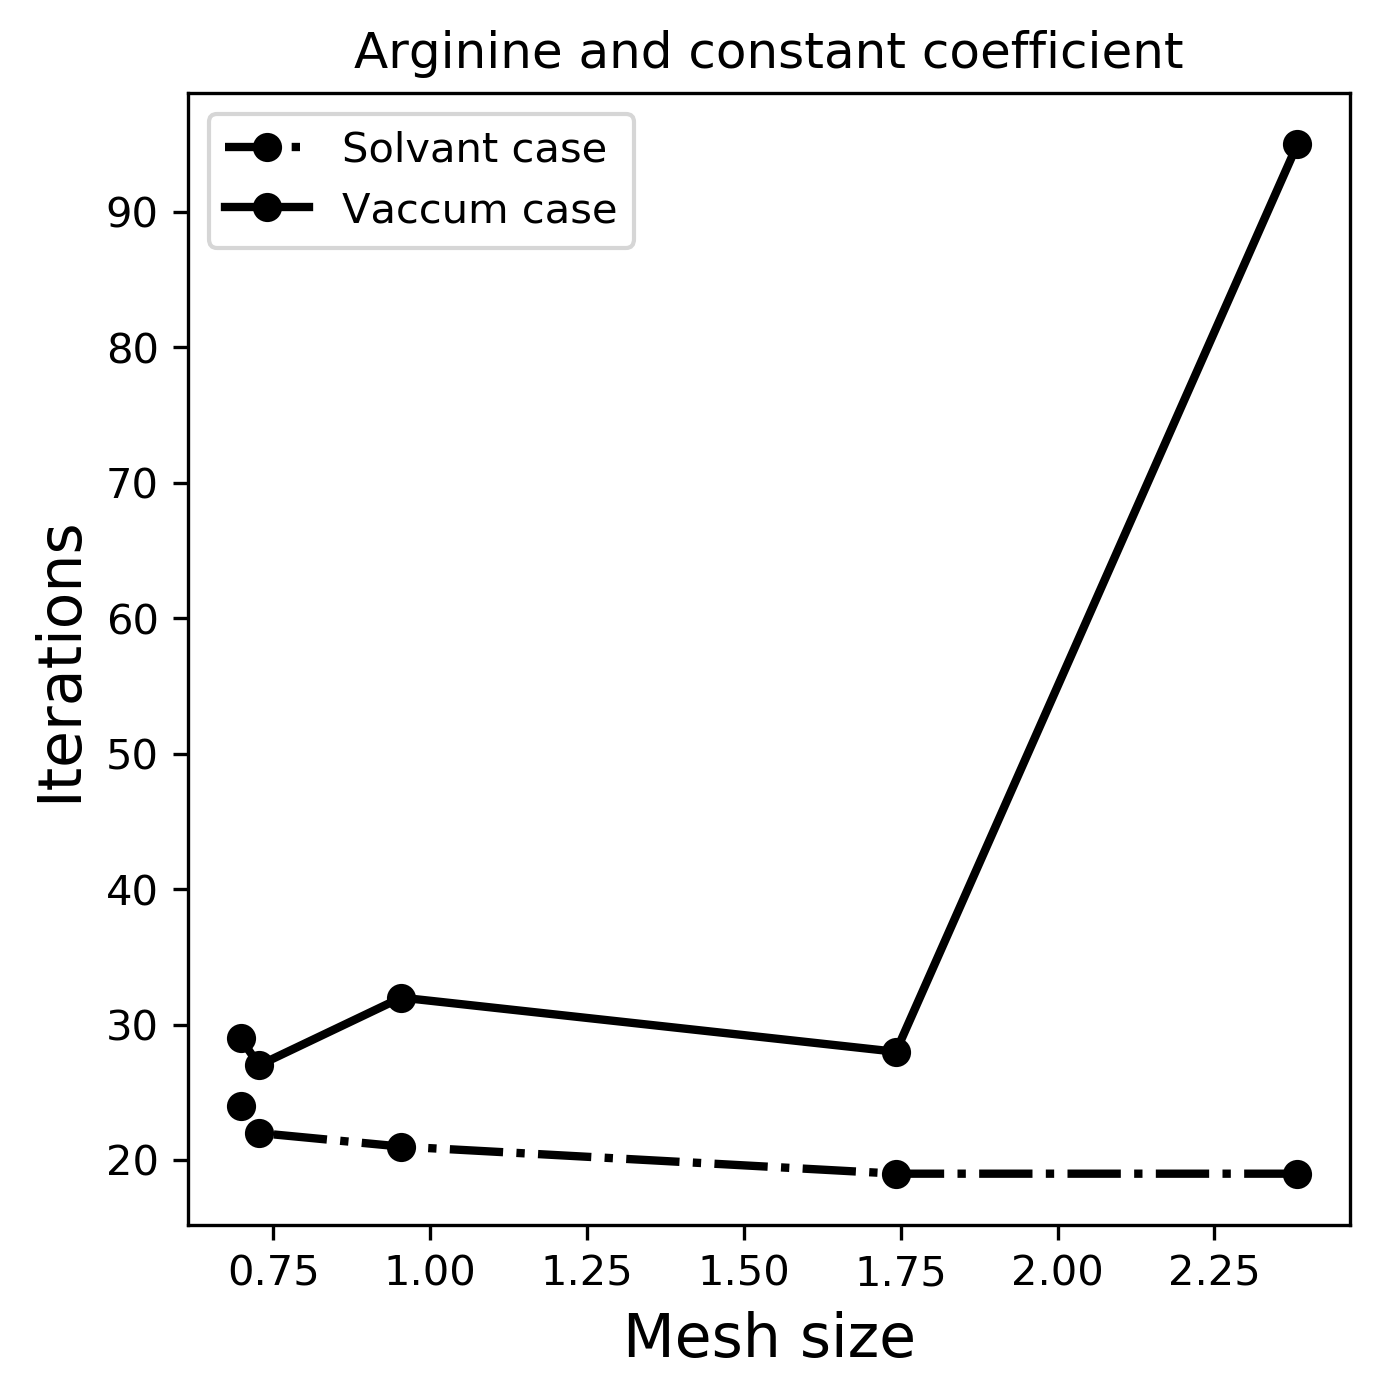
\includegraphics[width=\linewidth]{Hybrid_FEM_BEM_Arginine_const_coeff_iter.png}
  \caption{Iterations}
\endminipage\hfill
\minipage{0.45\textwidth}%
  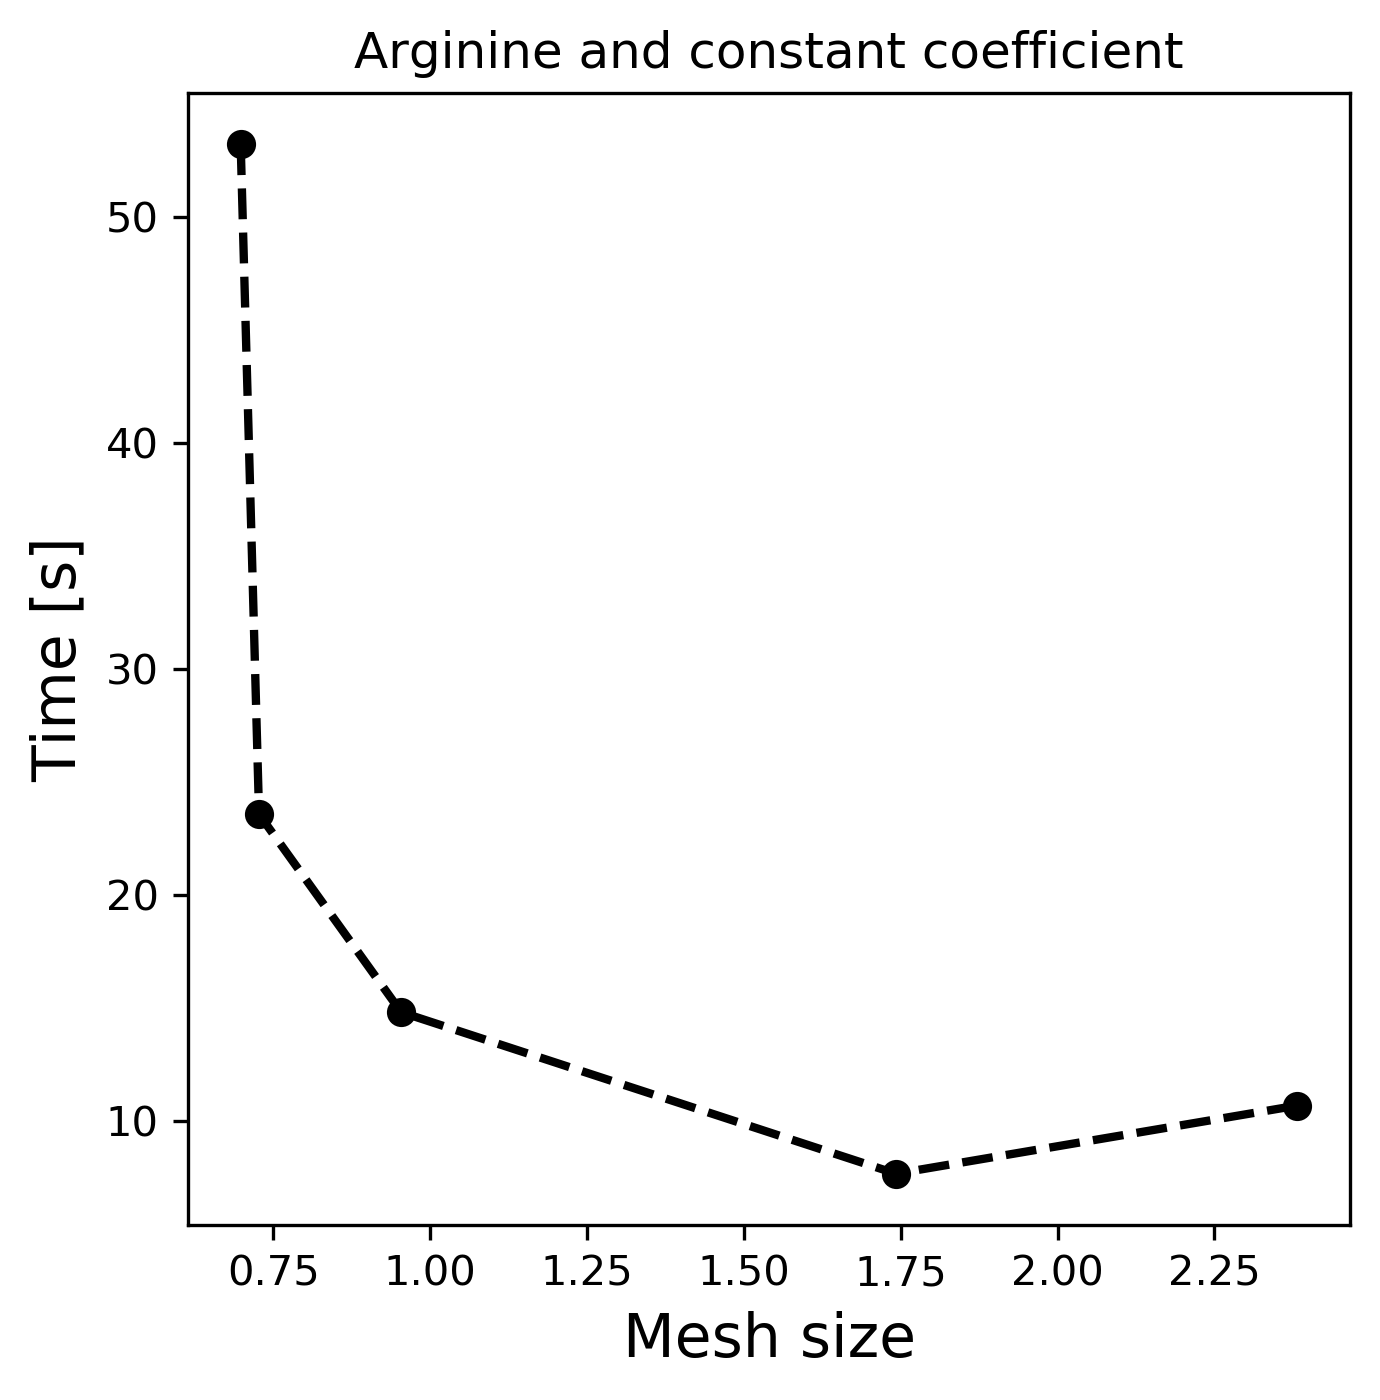
\includegraphics[width=\linewidth]{Hybrid_FEM_BEM_Arginine_const_coeff_time.png}
  \caption{Computational time}
\endminipage
\end{figure}
    \end{itemize}
    \item Compare computer time and iterations for FEM-BEM with standard and hybrid approaches, without preconditioner. Choose hybrid.
    \item Show performance of hybrid method with preconditioner.
\end{itemize}

\section*{\sffamily \Large Results with variable permittivity}

\begin{table}
\centering
\begin{tabular}{c|c|c}
&Mesh size & $\Delta G_{solv}$\\
&\AA       &  kcal/mol \\
\hline
\multirow{3}{*}{APBS}& 0.39$\times$0.39$\times$0.39 & -32.4042\\ 
&0.26$\times$0.26$\times$0.26 & -32.3375\\ 
&0.17$\times$0.17$\times$0.17 & -32.3413\\ 
\hline
&Mesh dens. & \\
&vert/\AA$^2$ & \\
\hline
%\multirow{5}{*}{Standard FEM-BEM}& 2 & -36.239\\
    & 2 & -36.239\\
Standard    & 4  & -33.129 \\
FEM-BEM    & 8  & -32.674 \\
    & 12 & -32.648 \\
    & 16 & -32.293 \\
\hline
%\multirow{5}{*}{Standard FEM-BEM}& 2 & -29.554\\
    & 2 & -29.554\\
Hybrid    & 4  & -33.766 \\
FEM-BEM    & 8  & -32.586 \\
    & 12 & -32.891 \\
    & 16 & -32.528 \\
\hline
\end{tabular}
\caption{}
\end{table}

    \begin{itemize}
        \item Standard FEM-BEM
\begin{figure}[!htb]
\minipage{0.45\textwidth}
  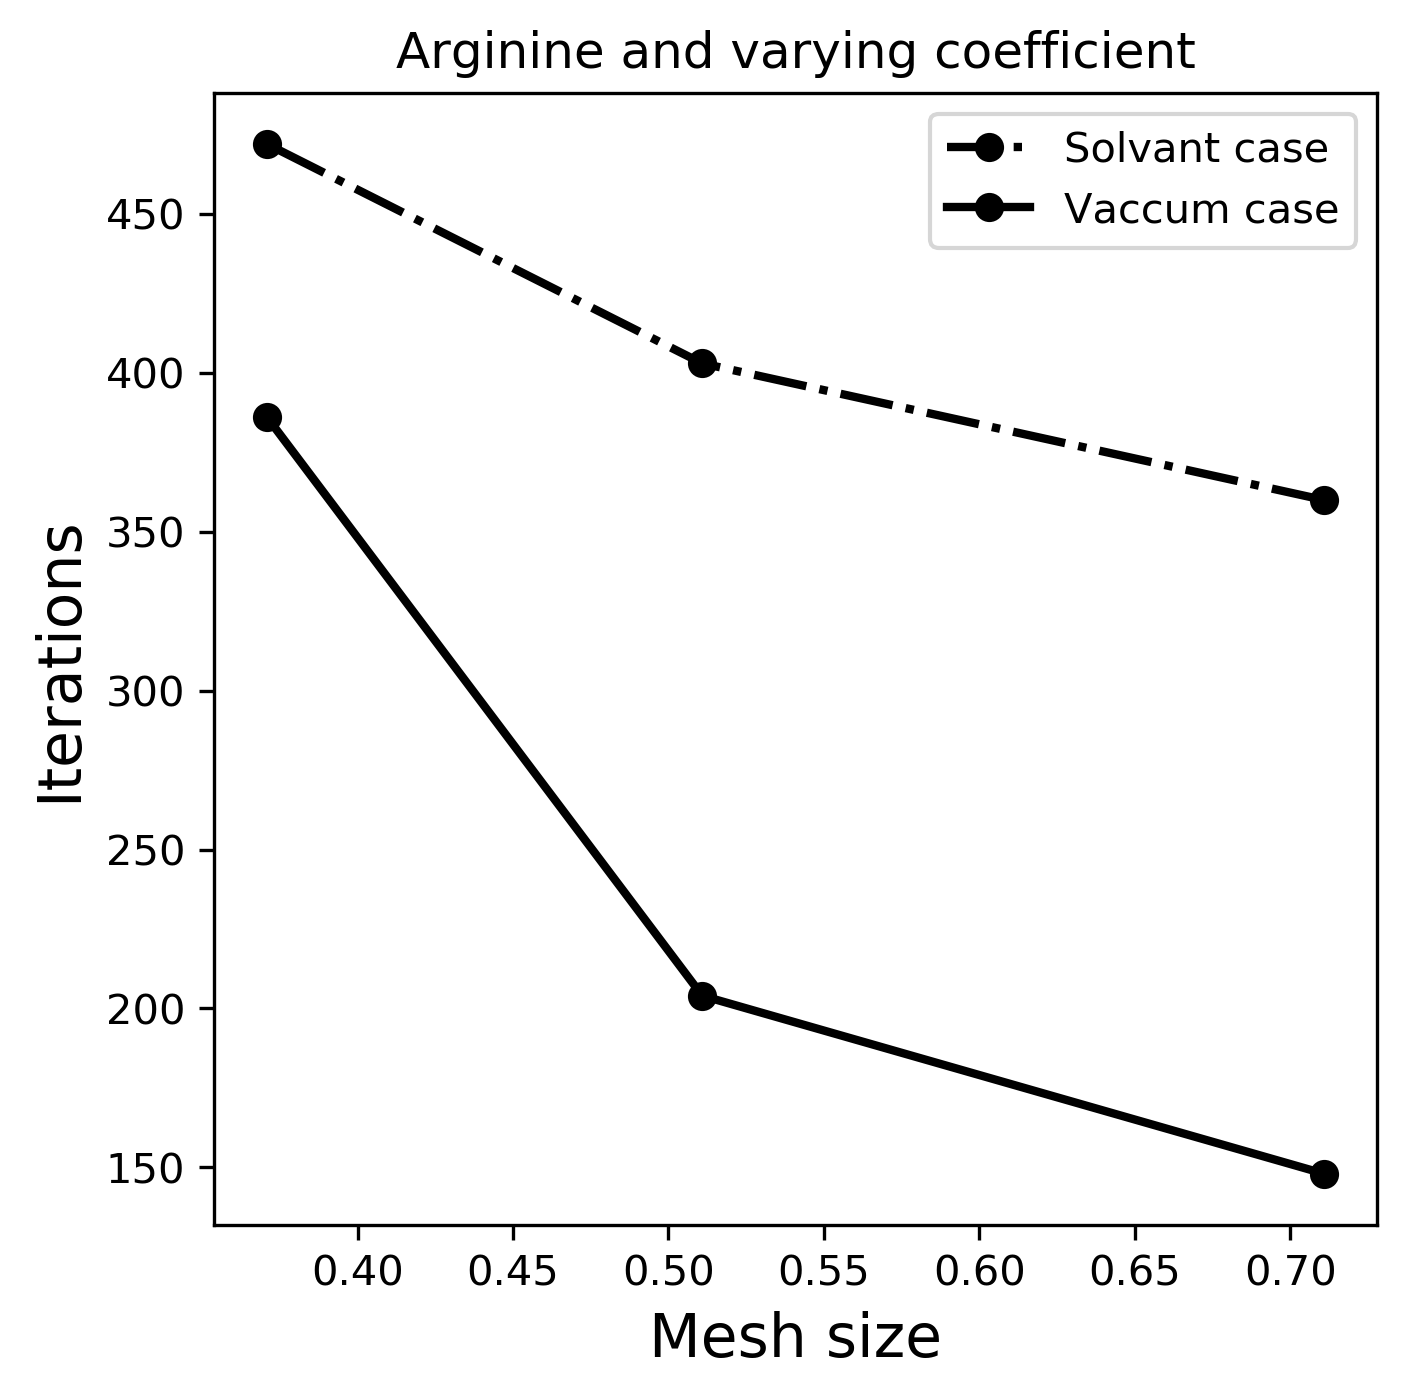
\includegraphics[width=\linewidth]{FEM_BEM_Sphere_varying_coeff_iter.png}
  \caption{Iterations}
\endminipage\hfill
\minipage{0.45\textwidth}%
  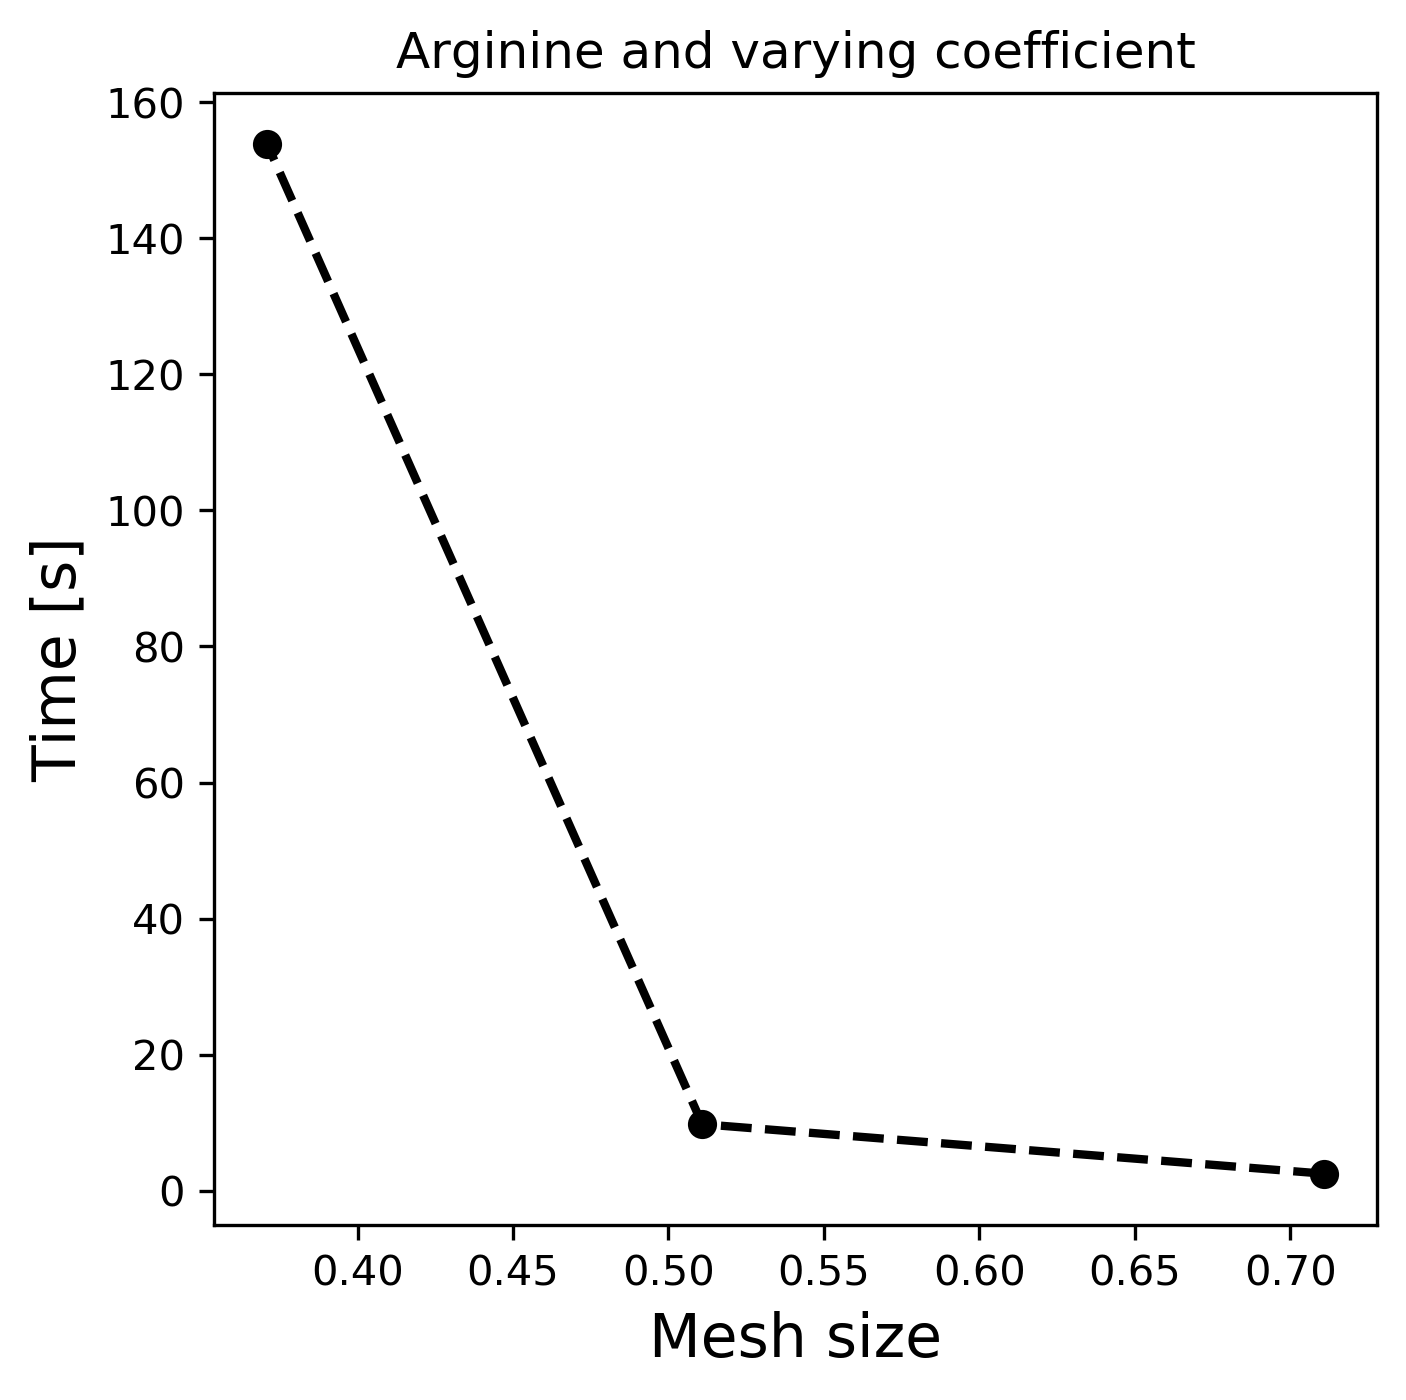
\includegraphics[width=\linewidth]{FEM_BEM_Sphere_varying_coeff_time.png}
  \caption{Computational time}
\endminipage
\end{figure}
        \item Hybrid FEM-BEM
\begin{figure}[!htb]
\minipage{0.45\textwidth}
  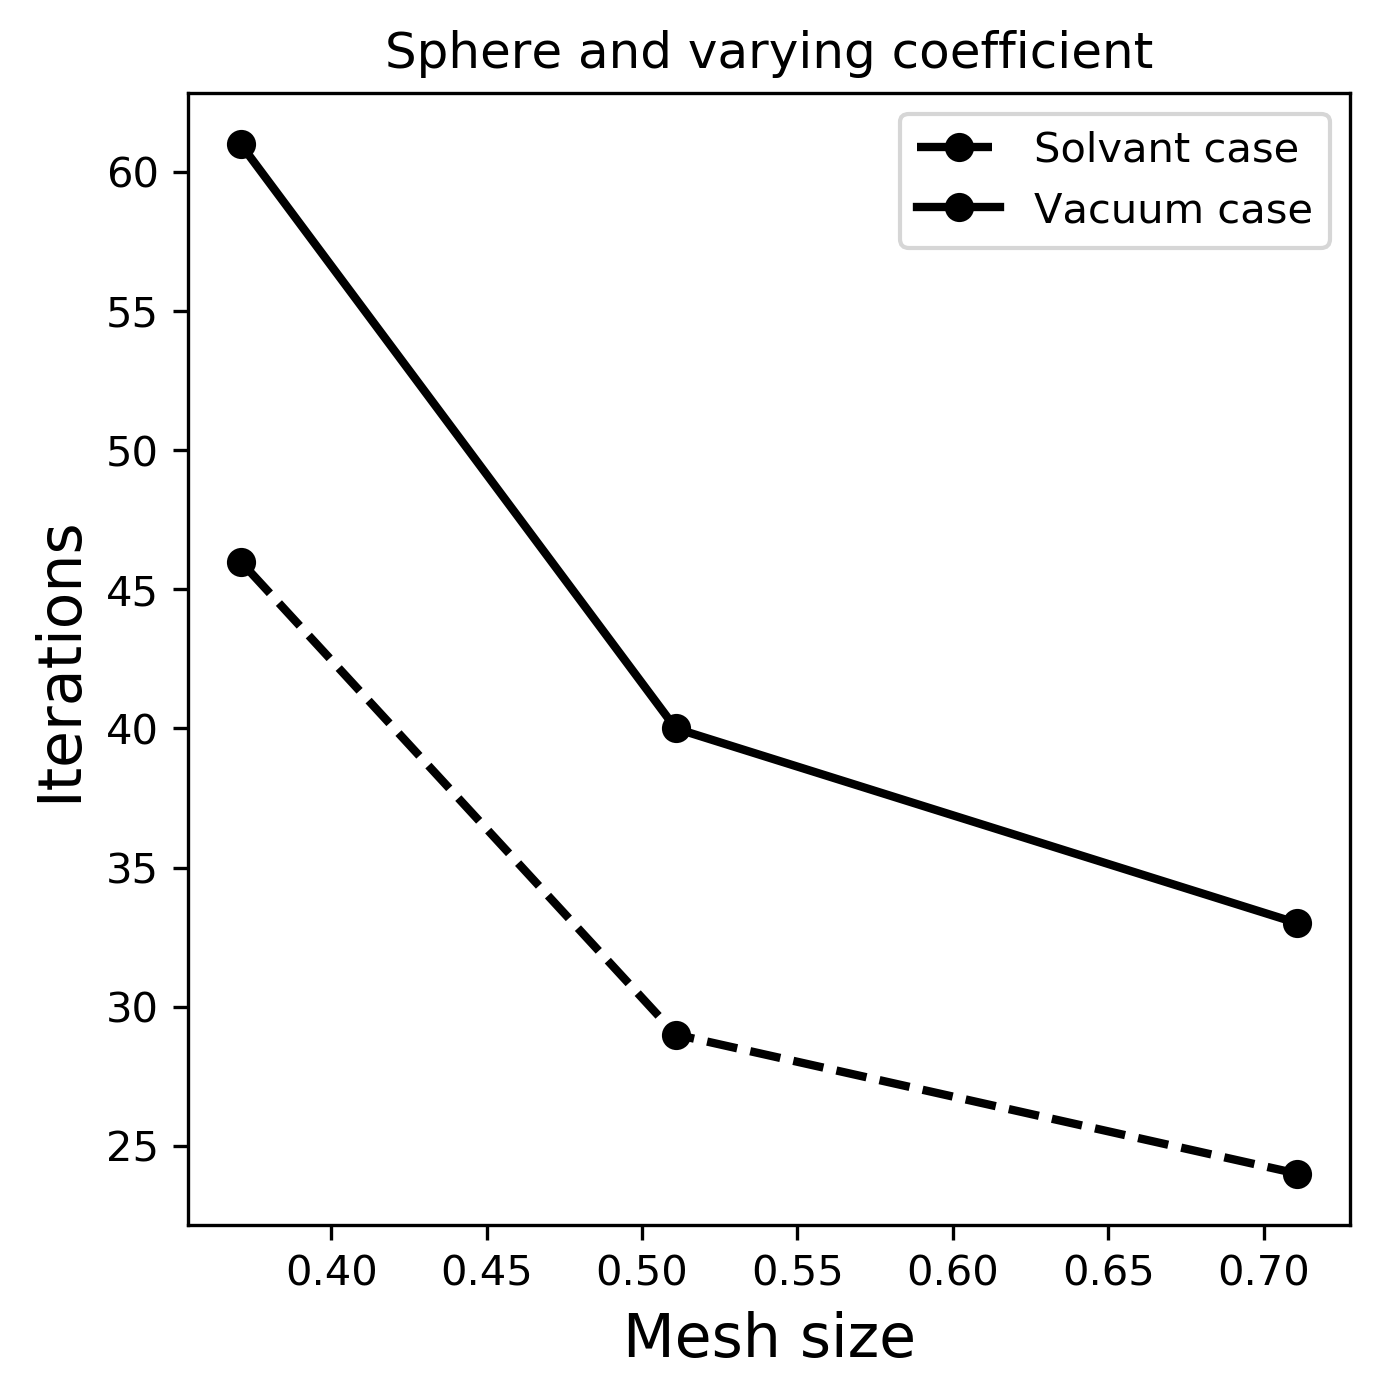
\includegraphics[width=\linewidth]{Hybrid_FEM_BEM_Sphere_varying_coeff_iter.png}
  \caption{Iterations}
\endminipage\hfill
\minipage{0.45\textwidth}%
  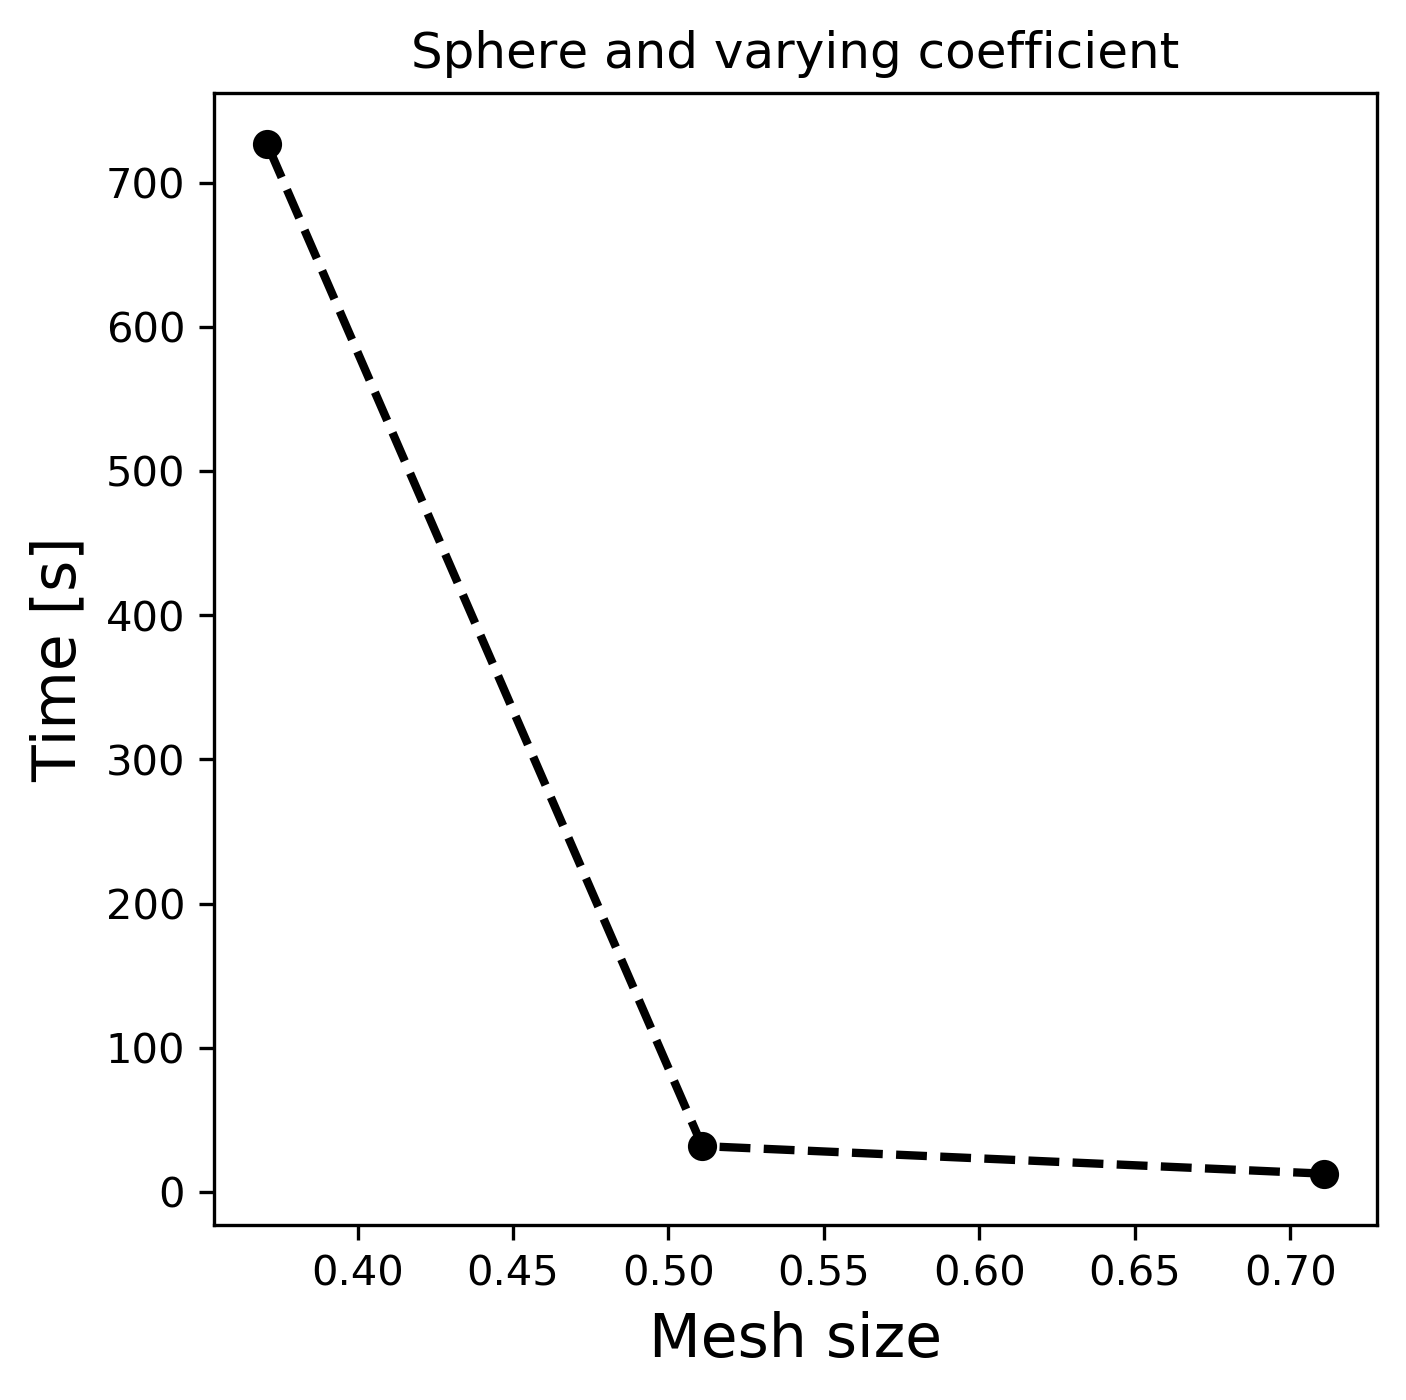
\includegraphics[width=\linewidth]{Hybrid_FEM_BEM_Sphere_varying_coeff_time.png}
  \caption{Computational time}
\endminipage
\end{figure}
    \end{itemize}

\subsection*{\sffamily \large Validation for a spherical cavity}

Compare solvation energy results of hybrid FEM-BEM with Delphi

\subsection*{\sffamily \large Convergence and performance for a molecular geometry}
\begin{itemize}
    \item Mesh refinement study using hybrid FEM-BEM and Delphi (if possible) on arginine or small protein. Check if they are converging to same result.
    \item Compare timings for equivalent error (if possible)
\end{itemize}

    \begin{itemize}
        \item Standard FEM-BEM
\begin{figure}[!htb]
\minipage{0.45\textwidth}
  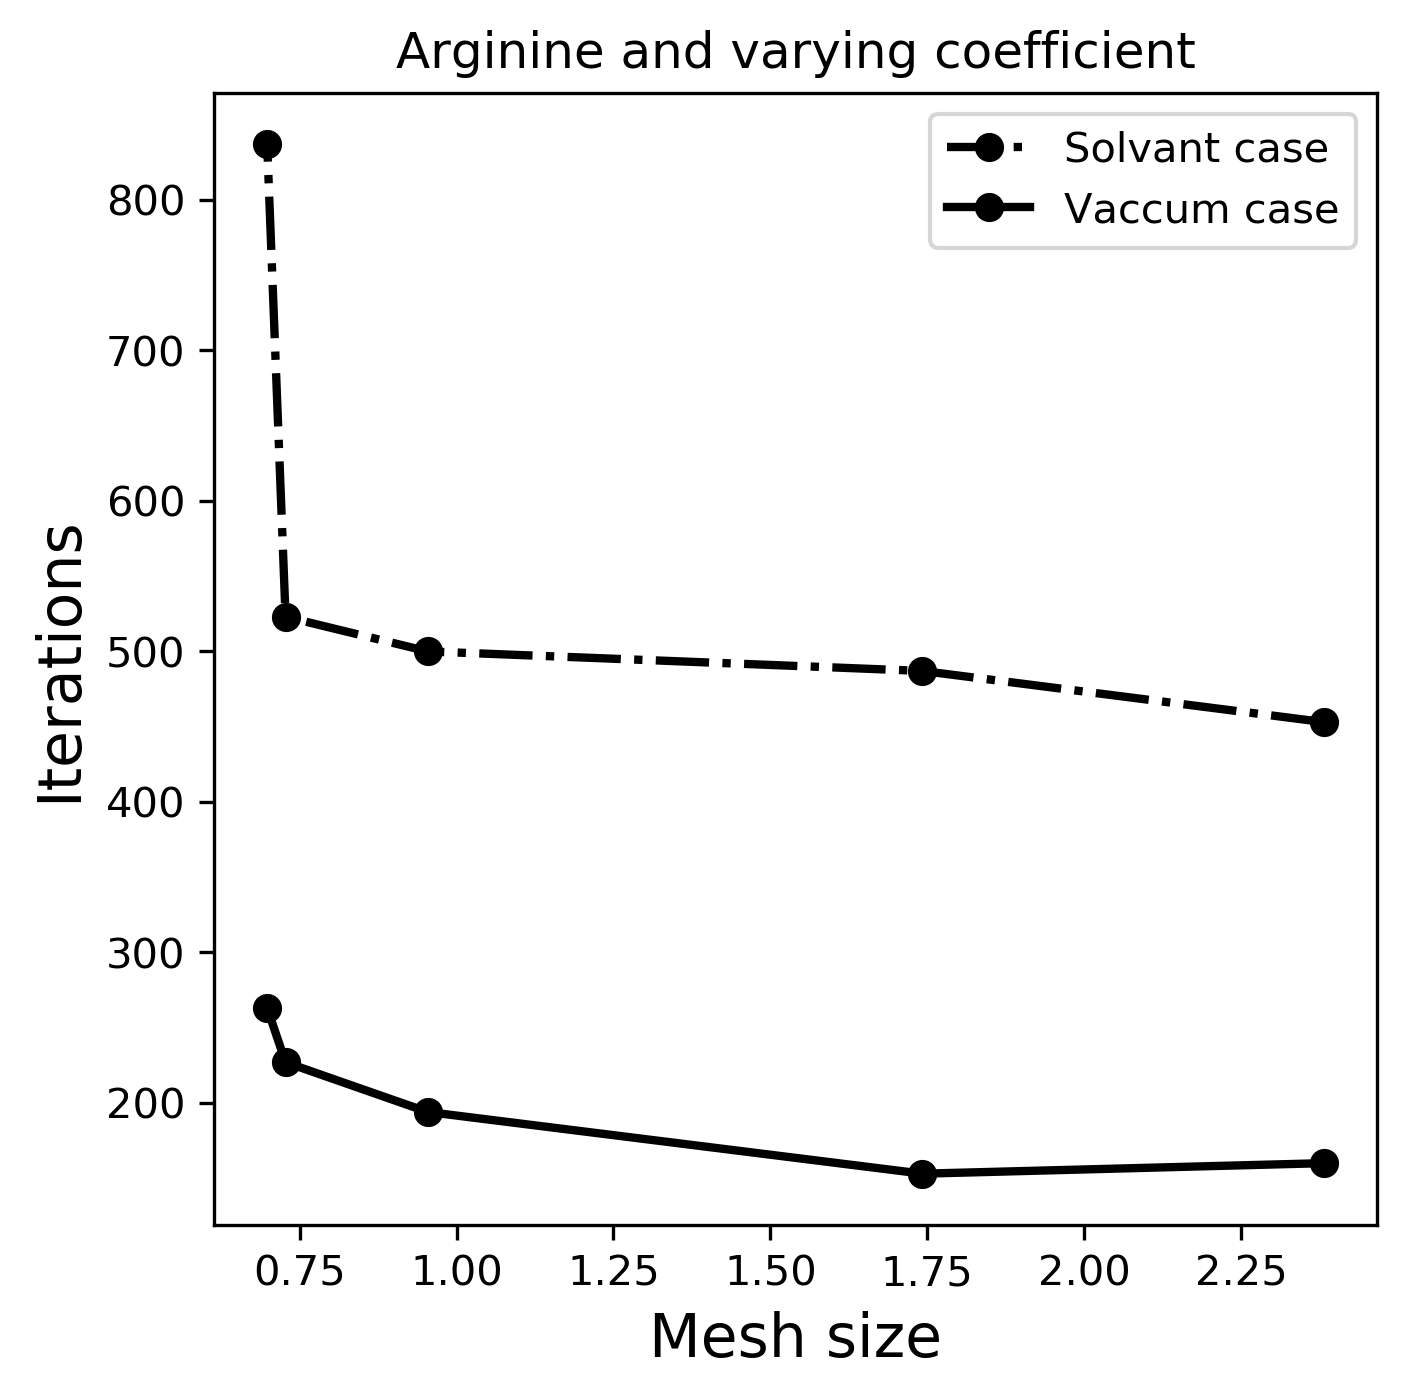
\includegraphics[width=\linewidth]{FEM_BEM_Arginine_varying_coeff_iter.png}
  \caption{Iterations}
\endminipage\hfill
\minipage{0.45\textwidth}%
  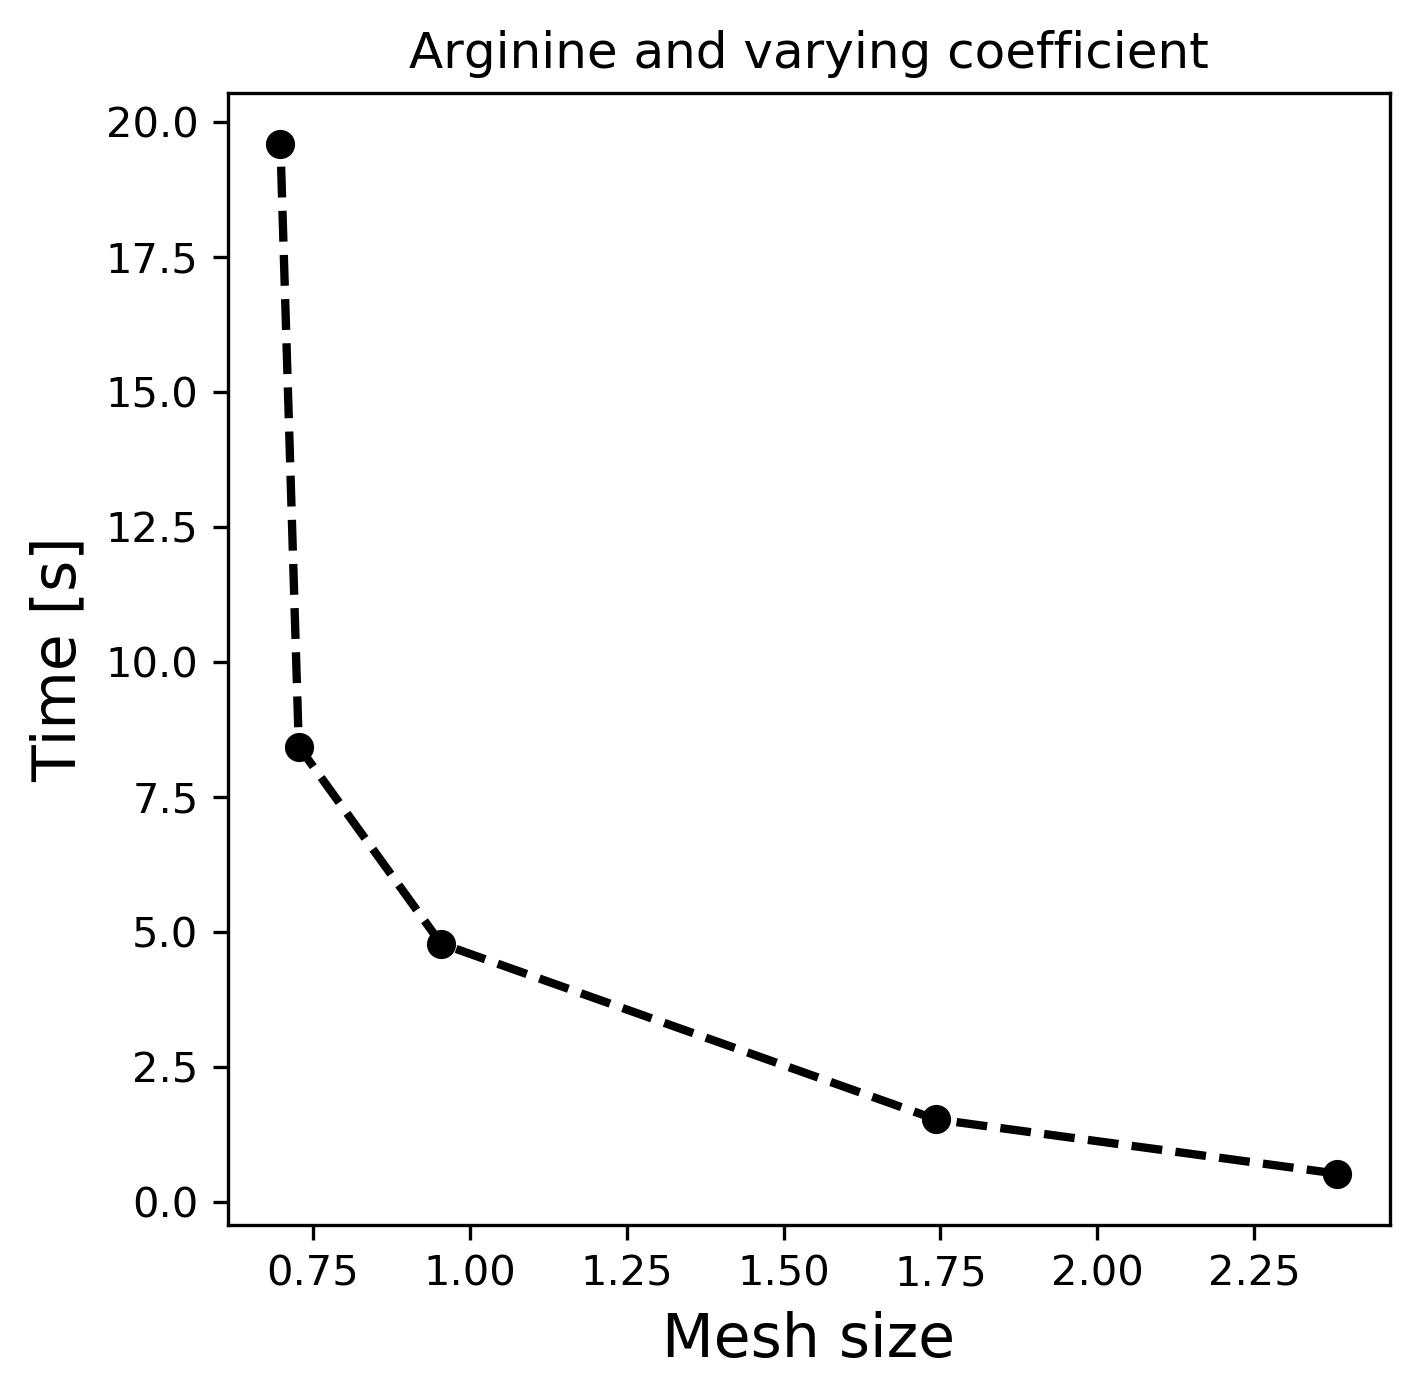
\includegraphics[width=\linewidth]{FEM_BEM_Arginine_varying_coeff_time.png}
  \caption{Computational time}
\endminipage
\end{figure}
        \item Hybrid FEM-BEM
\begin{figure}[!htb]
\minipage{0.45\textwidth}
  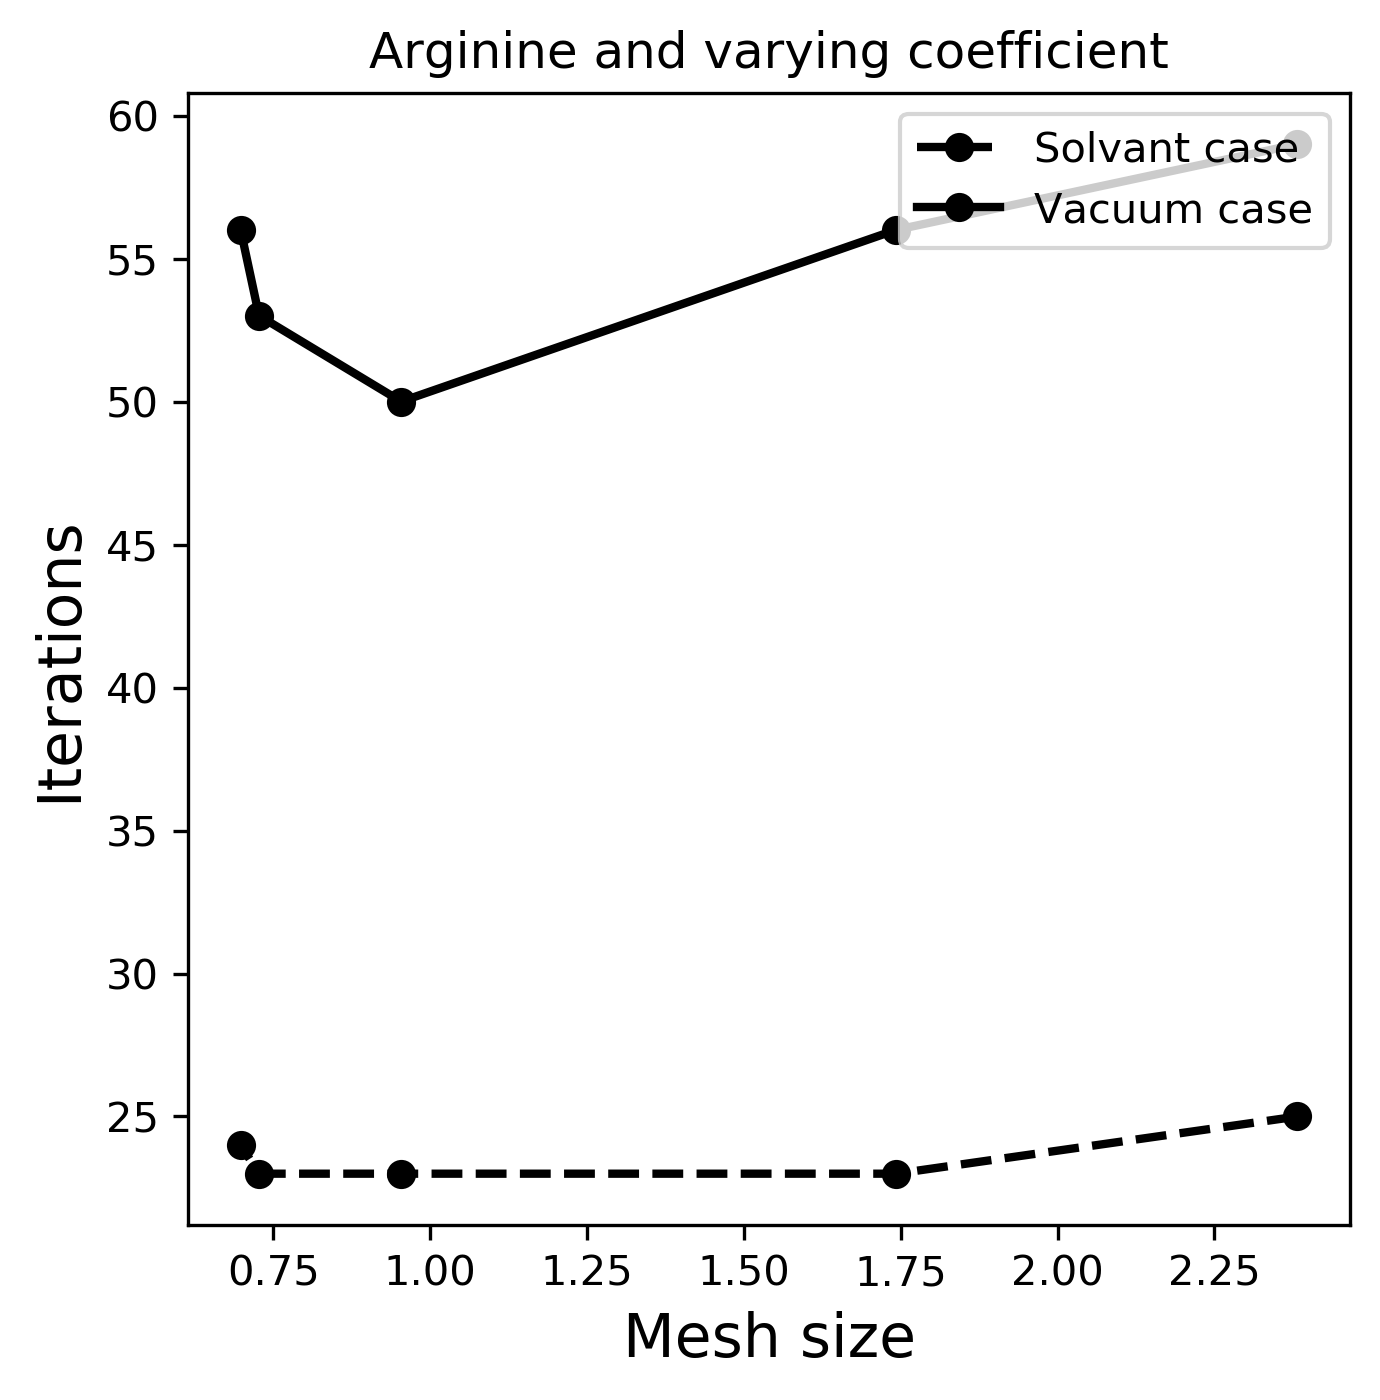
\includegraphics[width=\linewidth]{Hybrid_FEM_BEM_Arginine_varying_coeff_iter.png}
  \caption{Iterations}
\endminipage\hfill
\minipage{0.45\textwidth}%
  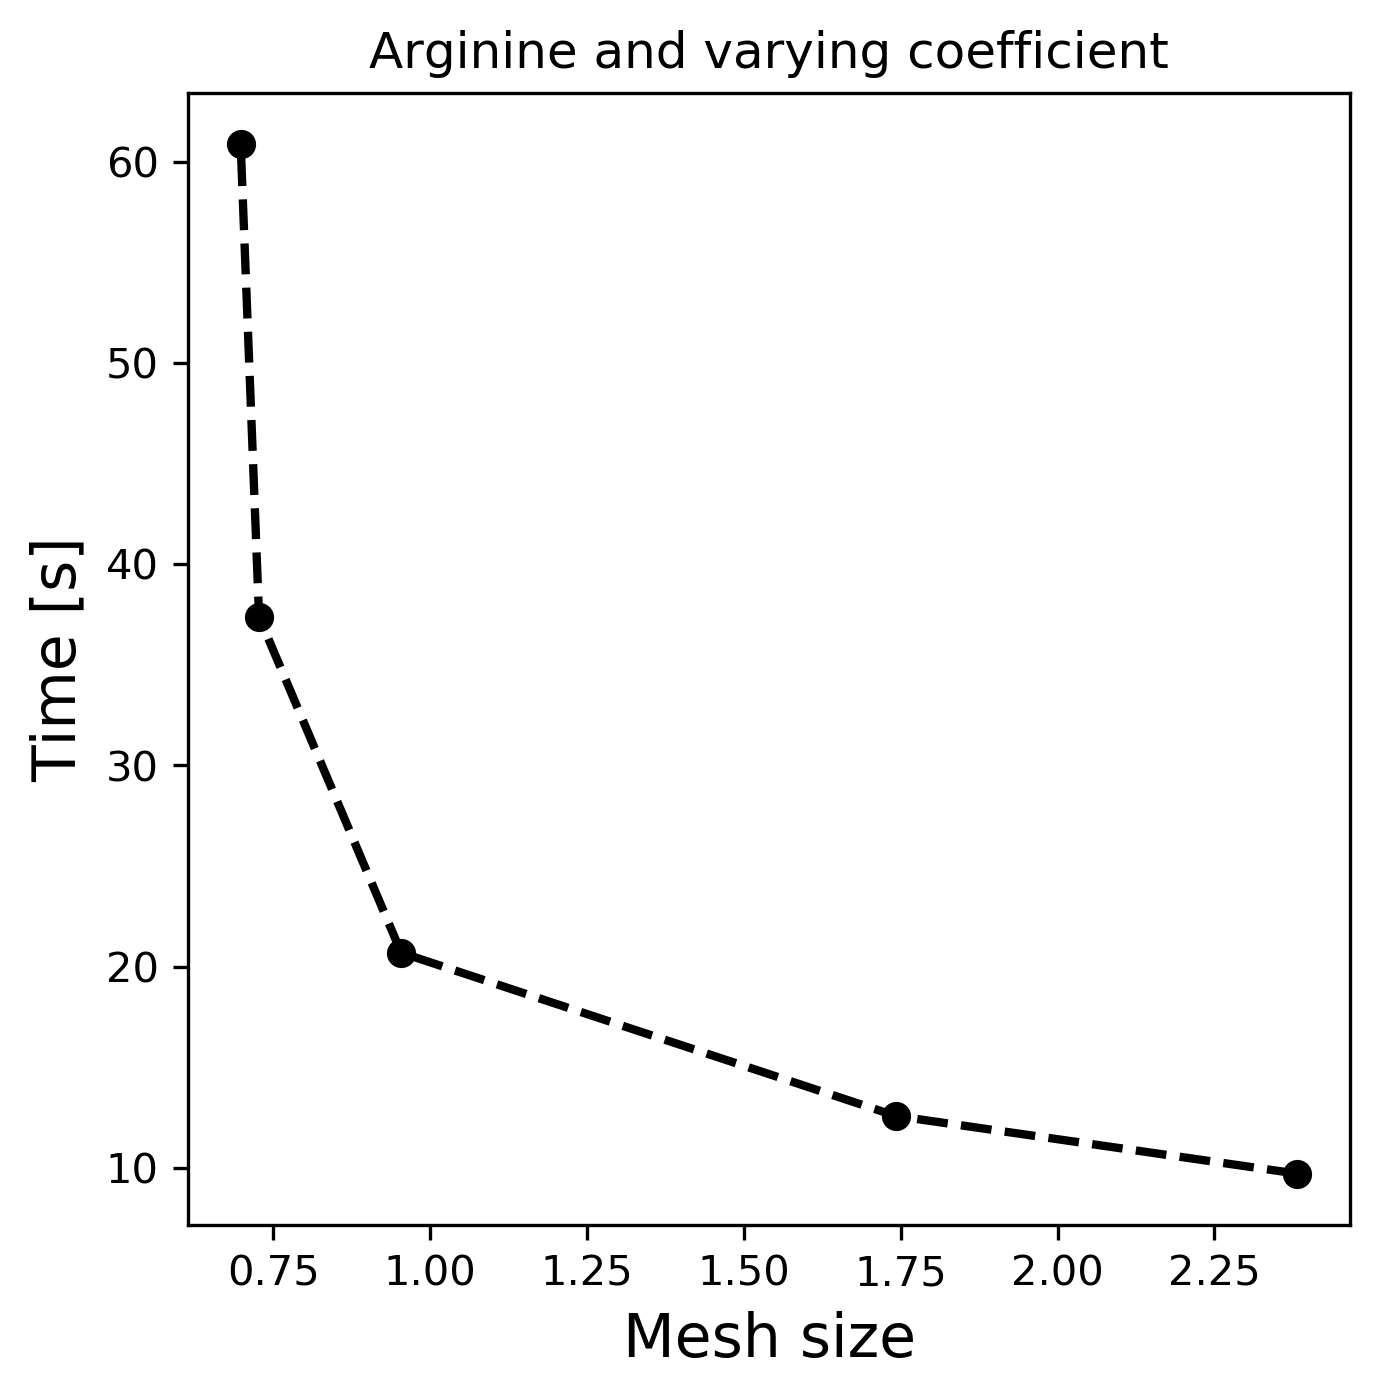
\includegraphics[width=\linewidth]{Hybrid_FEM_BEM_Arginine_varying_coeff_time.png}
  \caption{Computational time}
\endminipage
\end{figure}
    \end{itemize}

\subsection*{\sffamily \large Performance analysis for larger structures}

For a given mesh refinement, show solvation energy and timings using preconditioned hybrid FEM-BEM up to the biggest problem we can do on whatever computer we're using.
